\documentclass[final]{fhnwreport}         %[mode] = draft or final
%%---Main Packages-----------------------------------------------------------------------
\usepackage[english, ngerman]{babel}	%Mul­tilin­gual sup­port for LaTeX
\usepackage[T1]{fontenc}				      %Stan­dard pack­age for se­lect­ing font en­cod­ings
\usepackage[utf8]{inputenc}				  %Ac­cept dif­fer­ent in­put en­cod­ings
\usepackage{lmodern}                 %The newer Font-Set
\usepackage{textcomp}					      %LaTeX sup­port for the Text Com­pan­ion fonts
\usepackage{graphicx} 					      %En­hanced sup­port for graph­ics
\usepackage{float}						        %Im­proved in­ter­face for float­ing ob­jects
%\usepackage{ifdraft}                %Let you check if the doc is in draft mode

%%---Useful Packages---------------------------------------------------------------------
\usepackage[pdftex,dvipsnames,tables]{xcolor}  %Driver-in­de­pen­dent color ex­ten­sions for LaTeX
\usepackage{csquotes}                          %Simpler quoting with \enquote{}
\usepackage{siunitx} 					       %A com­pre­hen­sive (SI) units pack­age
\usepackage{listings}					       %Type­set source code list­ings us­ing LaTeX
\usepackage[bottom]{footmisc}			       %A range of foot­note op­tions
\usepackage{footnote}					       %Im­prove on LaTeX's foot­note han­dling
\usepackage{verbatim}					       %Reim­ple­men­ta­tion of and ex­ten­sions to LaTeX ver­ba­tim
\usepackage[textsize=footnotesize]{todonotes}  %Mark­ing things to do in a LaTeX doc­u­ment
\usepackage{lipsum}                            % Gives you access to blindtext

%%---Tikz Packages-----------------------------------------------------------------------
%\usepackage{standalone}
%\usepackage{tikz}
%\usepackage{circuitikz}
%\usetikzlibrary{arrows}
%\usetikzlibrary{calc}
%\usetikzlibrary{intersections}

%%---Math Packages-----------------------------------------------------------------------
\usepackage{amsmath}					    %AMS math­e­mat­i­cal fa­cil­i­ties for LaTeX
%\usepackage{amssymb}					  %Type­set­ting symbols (AMS style)
%\usepackage{array}						  %Ex­tend­ing the ar­ray and tab­u­lar en­vi­ron­ments
%\usepackage{amsthm}					    %Type­set­ting the­o­rems (AMS style)

%%---Table Packages----------------------------------------------------------------------
\usepackage{tabularx}					  %Tab­u­lars with ad­justable-width columns
%\usepackage{longtable}
\usepackage{multirow}					  %Create tab­u­lar cells span­ning mul­ti­ple rows
\usepackage{multicol}					  %In­ter­mix sin­gle and mul­ti­ple columns

%%---PDF / Figure Packages---------------------------------------------------------------
\usepackage{pdfpages}					  %In­clude PDF doc­u­ments in LaTeX
\usepackage{pdflscape}					  %Make land­scape pages dis­play as land­scape
%\usepackage{subfig}					    %Fig­ures di­vided into sub­fig­ures

%%---Other Packages----------------------------------------------------------------------
%\usepackage{xargs}              %De­fine com­mands with many op­tional ar­gu­ments


%%---Main Settings-----------------------------------------------------------------------
\graphicspath{{./graphics/}}			%Defines the graphicspath
%\geometry{twoside=false}				%twoside=false disables the "bookstyle"
\setlength{\marginparwidth}{2cm}
\overfullrule=5em						    %Creates a black rule if text goes over the margins => debugging

%%---User Definitions--------------------------------------------------------------------
%%Tabel-Definitions: (requires \usepackage{tabularx})
\newcolumntype{L}[1]{>{\raggedright\arraybackslash}p{#1}}    %column-width and alignment
\newcolumntype{C}[1]{>{\centering\arraybackslash}p{#1}}
\newcolumntype{R}[1]{>{\raggedleft\arraybackslash}p{#1}}					                        %loads all packages, definitions and settings	

\usepackage{listings}
%%%%% Bibliographie entweder im IEEE- oder im APA-Stil:
\usepackage[style=ieee,urldate=comp,backend=biber]{biblatex}
\usepackage{listings}
\usepackage{gensymb}
\usepackage{subcaption}
\usepackage{longtable,booktabs,array}
%\usepackage[style=apa,urldate=comp,backend=biber]{biblatex}
%%%%%
\addbibresource{literature/IP5_Literatur.bib}
\addbibresource{literature/references.bib}

\title{Traverse für autonomes Heben}  %Project Title
\author{IP5-Arbeit}    %Document Type => Technical Report, ...
\date{Windisch, Dezember 2024}               %Place and Date

\setcounter{tocdepth}{2}

\begin{document}
\pagenumbering{roman}	

%%---TITLEPAGE---------------------------------------------------------------------------
\selectlanguage{ngerman}                  %ngerman or english
\maketitle


\begin{figure}[H]
\centering

\includegraphics[width=0.7\textwidth]{graphics/stoica-ionela-CoNsEK5iHug-unsplash.png}\hfill%
\end{figure}

\begin{tabular}{@{}p{5cm} l}
Studentin/Student          &    Hoang Viet Nguyen\\
                           &    Alessandro Lenti\\[2ex]
                           
Betreuer/in                &    Christoph Stamm\\[2ex]
                           &    Hilko Cords\\[2ex]
Auftragsgeber              &    Ludwig System GmbH \& Co. KG\\[2ex]
\multicolumn{2}{@{}l}{Fachhochschule Nordwestschweiz, Hochschule für Technik}
\end{tabular}

\vspace*{4ex}
% Beispiel für Logo Industriepartner
\begin{tikzpicture}[remember picture,overlay,every node/.style={anchor=north east}]
  \node at (current page.north east) [xshift=-1cm, yshift=-0.5cm] {
\includegraphics[width=4cm]{graphics/LudwigSystem_Logo.png}};
  % Photo by Stoica Ionela on Unsplash
\end{tikzpicture}

\clearpage
			
%%---ABSTRACT----------------------------------------------------------------------------
\selectlanguage{ngerman}				%ngerman or english
\thispagestyle{empty}
\section*{Abstract}
\selectlanguage{ngerman}
Unser Partner, Ludwig System, entwickelt Traversen zur Balancierung schwerer Lasten wie Wände und Dächer. 
Die Befestigung dieser Lasten erfolgt bisher manuell, was eine gefährliche und zeitintensive Aufgabe darstellt. 
Zur Automatisierung dieses Prozesses sollte ein System entwickelt werden, das fähig ist, Anschlagspunkte automatisch erkennen zu können. 
In diesem Dokument wird ein Prototyp vorgstellt, der mittels AprilTags Anschlagspunkte identifiziert.
Dies wird durch die Posenschätzung der Marker erreicht und durch die Anordnung der Marker kann die Position und Rotation des Anschlagspunkt in Echtzeit berechnet werden und Ausgegeben werden.
Die Implementierung konnte die meisten Anforderungen von Kunden erfüllen, ausser die Genauigkeiten zur Neigung, da keine Tests durchgeführt werden konnten.
Weiters konnte nicht die Zuverlässigkeit des Systems bei Wetter evaluiert werden. 
Zurzeit ist die Latenz in der Implementation zu hoch. 
\vspace{2ex}

\textbf{Keywords:}

Fiducial Marker, Apriltags, ArUco, 3D Lokalisierung, OpenCV, Python

\clearpage




%%---TABLE OF CONTENTS-------------------------------------------------------------------	
\selectlanguage{ngerman}				%ngerman or english
\tableofcontents
\clearpage


\cleardoublepage

%%---Einleitung--------------------------------------------------------------------------
\pagenumbering{arabic}
\section{Einleitung}

Der Einsatz von Kränen ist auf Baustellen unerlässlich, um schwere Lasten zu bewegen.
Aktuell erfordert das Anhängen dieser Lasten an den Kran manuelle Arbeit durch Bauarbeiter.
Dies ist besonders zeitaufwendig, wenn der Schwerpunkt der Last ungleichmässig verteilt ist 
und führt häufig dazu, dass die Last mehrmals abgesetzt und angehoben werden muss, um sie 
korrekt auszurichten. Dies verursacht erhebliche Wartezeiten für andere Teammitglieder. 
Die Firma Ludwig System hat eine automatische Traverse entwickelt, die das Ausrichten und 
Positionieren der Last erleichtert, jedoch muss auch mit dieser aktuellen Version ein Mitarbeiter 
die Last manuell an die Traverse anhängen.

\begin{figure}[H]
    \centering
    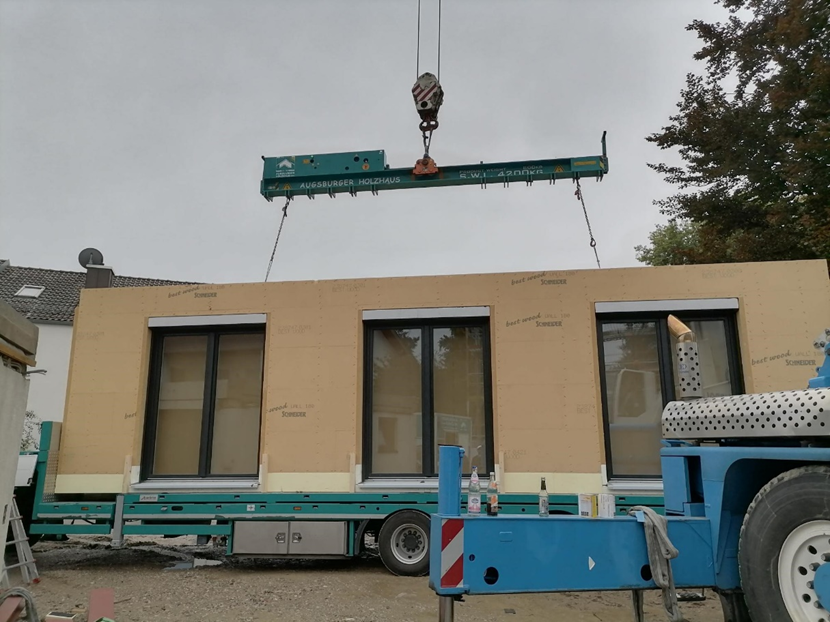
\includegraphics[width=\linewidth]{traverse.png}
    \caption{Ludwig Traverse im Einsatz}
\end{figure}

Die nächste Generation der Traverse zielt darauf ab, den Prozess der Lastenaufhängung zu automatisieren.
Ludwig System arbeitet derzeit intensiv an dieser Entwicklung und hat bereits Prototypen eines Greifarms 
erstellt, der dazu bestimmt ist, die Anschlagspunkte automatisch zu heben. Ein entscheidender Schritt in diesem 
Prozess ist die präzise Berechnung der Position dieser Anschlagspunkte.

Auf den ersten Blick erscheinen moderne Lösungen aus dem Bereich des maschinellen Lernens als ideal für diese Aufgabe. 
Jedoch besteht die Herausforderung darin, dass für das Training eines effektiven Modells eine umfangreiche Menge an Daten 
benötigt wird, die derzeit noch nicht ausreichend verfügbar ist. Zusätzlich erfordert die Anwendung solcher Technologien weiterführende 
Forschungen, um aus den erkannten Anschlagspunkten die Entfernung und Ausrichtung relativ zur Kamera zu bestimmen. Diese Berechnungen werden 
noch komplexer, wenn die Anschlagspunkte in verschiedenen Dimensionen vorliegen, was eine zusätzliche Anpassung und Verfeinerung der Algorithmen 
erfordert.

Ein weiterer Ansatz ist die Verwendung von Passmarkern. Diese Marker haben den Vorteil, dass sie in standardisierten Grössen verfügbar sind, was 
ihre Erkennung erleichtert \cite{astrobee2023}. Durch die Analyse der Eckpunkte eines Markers kann die Position relativ zur Kamera bestimmt werden 
\cite{localizationSystem}. Zusätzlich ermöglicht die Codierung einer eindeutigen ID auf dem Marker die Feststellung seiner Ausrichtung. Theoretisch
erlaubt dies dem Kranführer, die Traverse präzise auszurichten. Der Einsatz solcher Markierungssysteme wird bereits in der Robotik erfolgreich zur 
Positions Bestimmung von Objekten genutzt, was deren Effektivität und Zuverlässigkeit unterstreicht \cite{localizationSystem}.

Die Arbeiten von \cite{yong_object_2023} und \cite{zhou_image-based_2021} zeigen, dass mithilfe von Machine-Learning-Methoden Objekte erfolgreich identifiziert werden können.
Da uns jedoch die nötigen Daten fehlen, um KI zur Bestimmung von Anschlagpunkten einzusetzen, fokussieren wir uns in dieser Arbeit auf Fiducial Marker. Diese bieten den Vorteil, 
dass ihre Ausrichtung und Grösse im Voraus festgelegt werden können, was Berechnungen vereinfacht. Für unsere Anwendung haben wir AprilTags gewählt, da sie in Vergleichstests höhere 
Genauigkeiten als AruCo-Marker erzielen. Um die Position des Anschlagpunktes zu bestimmen, nutzen wir ein Kreuzmuster aus vier AprilTags, bei dem der Anschlagpunkt zentral in der Mitte liegt.
Tests und ein Prototyp zeigen, dass die Abweichungen innerhalb der vom Kunden geforderten Toleranzgrenzen liegen, wodurch unser Ansatz eine praktikable Lösung darstellt.

\begin{figure}[H]
    \centering
    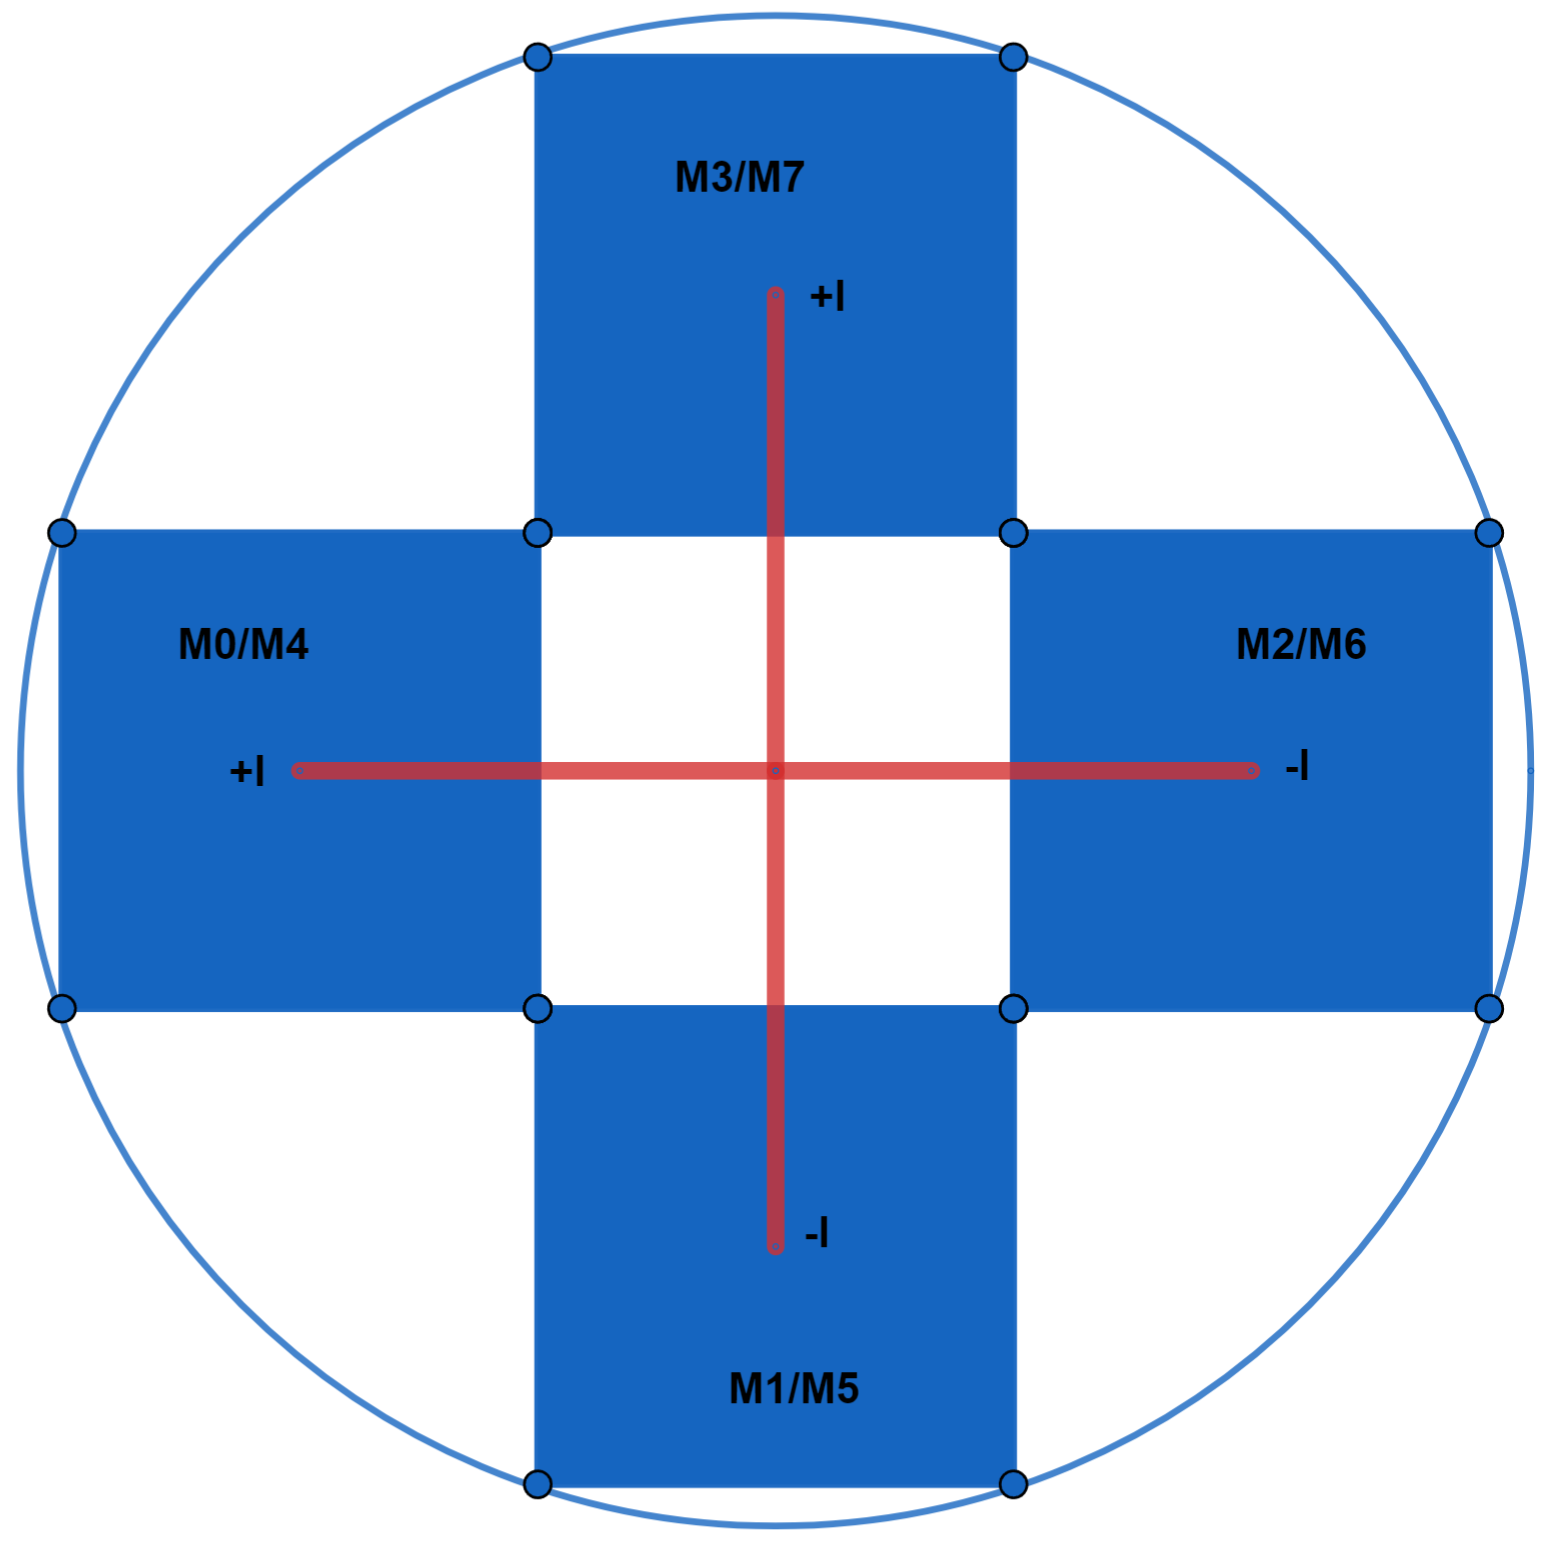
\includegraphics[width=0.5\linewidth]{graphics/marker_anordnung.png}
    \caption{Kreuzmuster zur Positions Bestimmung}
\end{figure}


In den folgenden Kapiteln schaffen wir zunächst eine Grundlage, um das Problem und unsere Lösung besser zu verstehen. Anschliessend 
widmen wir uns Projekten, die ähnliche Herausforderungen bereits behandelt haben.

Darauf aufbauend präsentieren wir unsere Konzepte zunächst theoretisch, bevor wir zur praktischen Implementierung 
übergehen. Abschliessend stellen wir unsere Ergebnisse vor, diskutieren mögliche Alternativen zur Problemlösung und 
zeigen auf, wie wir unsere Ansätze weiter verbessern könnten.




%%---TEXT--------------------------------------------------------------------------------
\section{Grundlagen}
Wir beginnen mit einem Überblick über das Problem und die Zielgruppe unserer Kunden.
Anschliessend führen wir grundlegende Begriffe ein, die für das Verständnis unseres Projekts
wichtig sind. Im nächsten Schritt betrachten wir ähnliche Projekte, die vergleichbare Herausforderungen adressieren.
Da wir Fiducial Marker zur Erkennung der Anschlagpunkte verwenden, erläutern wir die Grundlagen zur 
Erkennung dieser Marker sowie zur Bestimmung ihrer Position relativ zur Kamera. Wir werden ausserdem eine Einführung in 
Kamera-Hardware geben und erläutern, warum deren Kalibrierung vor den Berechnungen von entscheidender Bedeutung ist.
Abschliessend stellen wir die Frameworks vor, die im Projekt verwendet wurden.

\subsection{Problemstellung}
Ludwig System, ein Hersteller von Werkzeugen für Baustellen, entwickelt derzeit eine autonome Traverse. Damit diese 
Traverse autonom agieren kann, müssen drei wesentliche Ziele erreicht werden: die automatische Erkennung einer Last, 
die mechanische Ausrichtung der Traverse basierend auf der erkannten Last und den Anschlagspunkten sowie die Verriegelung 
der Haken an den Anschlägen. Während Ludwig System die Entwicklung der letzten beiden Schritte übernimmt, konzentriert sich
unsere Arbeit auf die Erfüllung des ersten Schrittes. Hierbei geht es um die Auswahl geeigneter Sensoren und die Implementierung
praktikabler Methoden, die es der Traverse ermöglichen, Lasten und Anschlagspunkte zu erkennen. Zur besseren Verständlichkeit der 
folgenden Ausführungen werden im nächsten Schritt die relevanten Schlüsselbegriffe definiert.


\subsubsection{Anwendungsdomäne}
Das Abhängen von Lasten per Hand ist nicht nur zeitaufwendig, sondern oft auch gefährlich. 
Ludwig System bietet mit ihren funkgesteuerten Lasthaken eine innovative Lösung, 
die diese Arbeit deutlich erleichtert. Diese Haken ermöglichen es den Mitarbeitenden, 
Lasten aus sicherer Entfernung anzuheben und auszubalancieren. Besonders beliebt ist 
die Traverse, die speziell für den Transport von Dachelementen und Wänden entwickelt wurde. 
Allerdings müssen aktuelle Versionen noch manuell an die Last befestigt werden, 
was besonders bei hohen Wänden zeitaufwendig und gefährlich sein kann. 
Abbildung \ref{fig:ludwig} illustriert die Nutzung der Traverse und des Haken.

\begin{figure}[H]
    \centering
    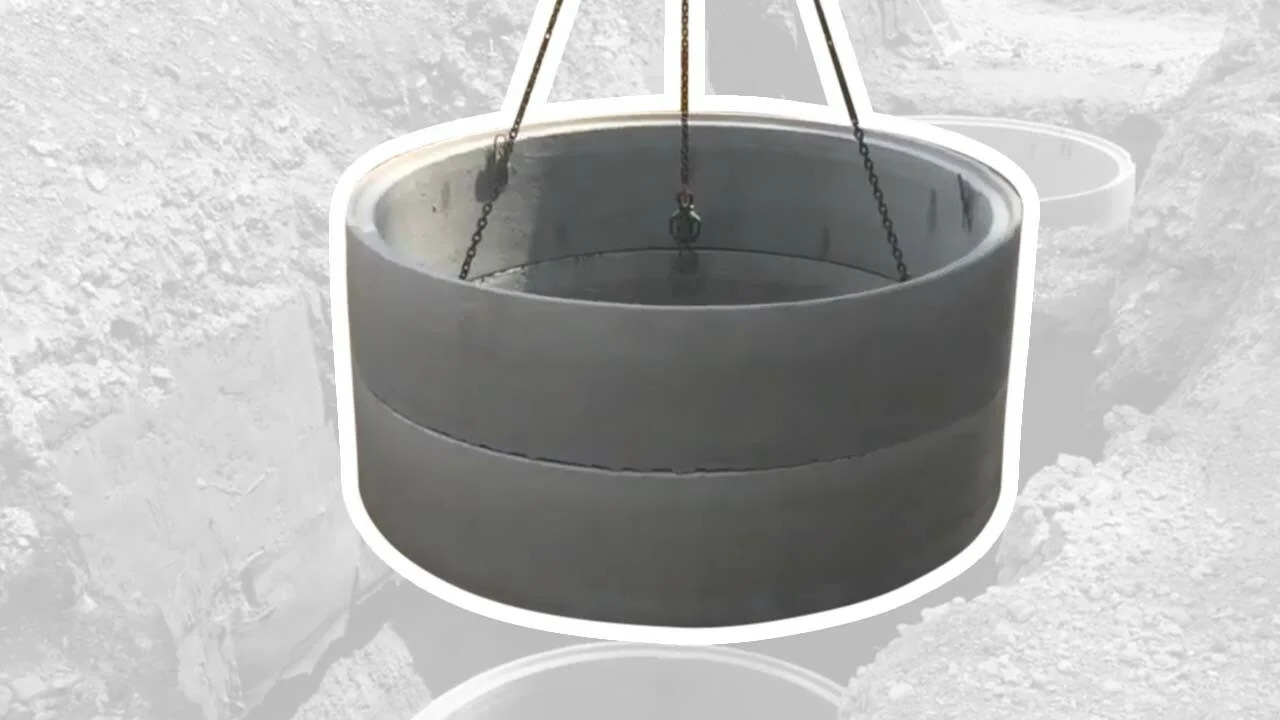
\includegraphics[width=0.5\textwidth]{graphics/Betonelement.jpg}\hfill%
    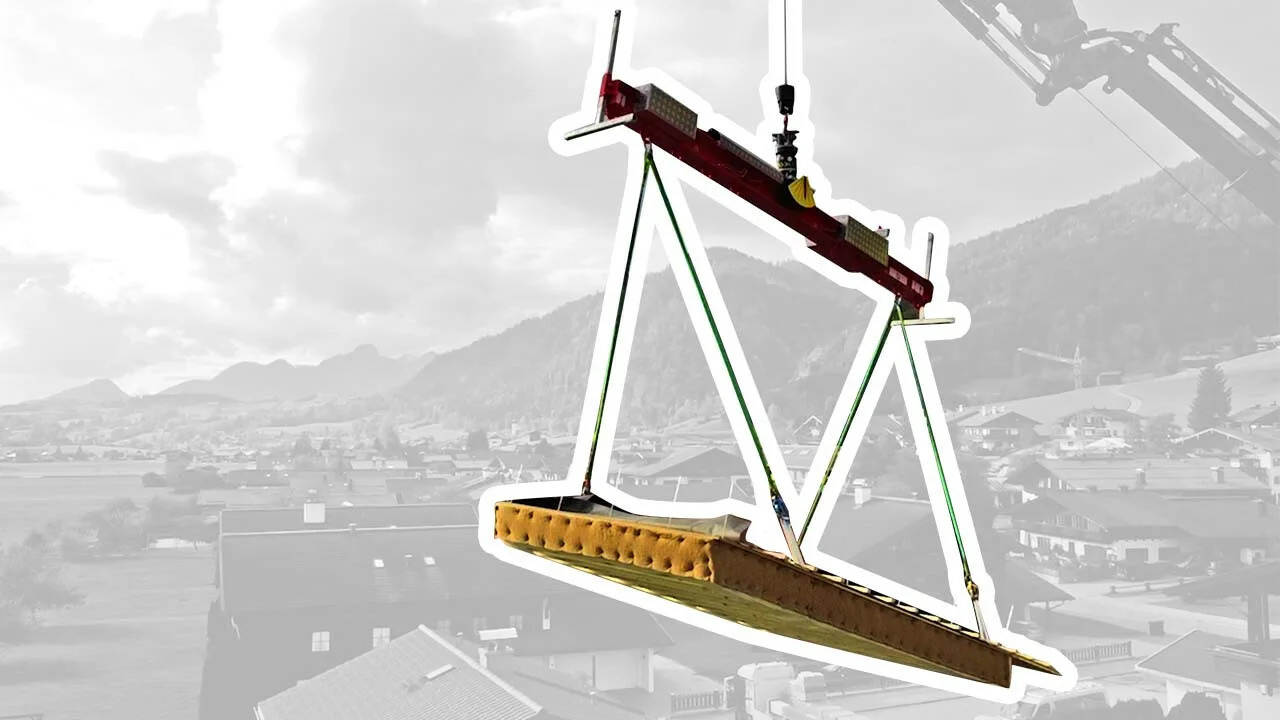
\includegraphics[width=0.5\textwidth]{graphics/Traverse.jpg}
    \caption{Ludwig Hook und Ludwig Traverse}
    \label{fig:ludwig}
\end{figure}

\subsubsection{Last}
Unter Lasten sind vor allem Fertigstrukturen wie z.B. Fertig erstellte Wände oder Dächer. 
Lasten haben maximal 2 Anschlagspunkte, welche einen Abstand von 1m bis 6m zueinander haben.
Diese Anschlagspunkte können auf unterschiedliche Höhen sein, wie z.B. bei Dächern welche eine
Neigung besitzen.

\subsubsection{Traverse}
Die LudwigTraverse ist eine Spezialtraverse, die speziell für den Lastausgleich entwickelt 
wurde. Sie erweist sich insbesondere dann als nützlich, wenn die Anschlagspunkte 
falsch positioniert sind und dadurch der Schwerpunkt der Last nicht korrekt berücksichtigt wird. 
Dies kann zu einer schrägen Ausrichtung beim Anheben der Last führen \cite{ludwigTraverse}.

\begin{figure}[H]
    \centering
    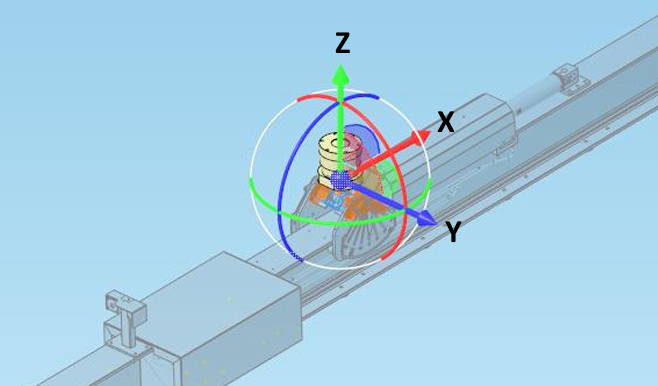
\includegraphics[width=0.5\linewidth]{graphics/Traverse_Rotationen.PNG}
    \caption{Koordinatensystem der Ludwig System Traverse}
    \label{fig:traverse}
\end{figure}

Abbildung \ref{fig:traverse} zeigt das linkshändige Koordinatensystem der Traverse.
Die Traverse hat Dimensionen (Länge × Breite × Höhe) von 500 cm × 70 cm × 50 cm.
Dabei wird fortan die Rotation um die Y-Achse der Traverse als Neigen definiert und die Rotation 
um die Z-Achse der Traverse als Rotieren definiert.

\subsection{Stand der Forschung}
Das Problem der Erkennung von Anschlagpunkten kann auf die Disziplin der Objektdetektion reduziert werden.
In der Arbeit von \cite{yong_object_2023} wird eine Methode vorgestellt, um mithilfe von Deep-Learning-Algorithmen 
in Kombination mit Ultraschallsensoren Unfälle auf Baustellen zu vermeiden. Diese Technologie wird genutzt, um die
Umgebung eines Krans zu überwachen und bei Bedarf einzugreifen. Das System integriert dabei eine Objekterkennung mit
einer Internet-Protokoll (IP)-Kamera zur Identifikation von Bauarbeitern im Gefahrenbereich und Ultraschallsensoren zur 
Messung von Abständen zu Hindernissen. Die Feldtests der entwickelten Lösung zeigten vielversprechende Ergebnisse, die 
zur Erhöhung der Sicherheit auf Baustellen beitragen können.


Eine weitere Arbeit, die den Nutzen von maschinellem Lernen auf Baustellen untersucht, ist \cite{zhou_image-based_2021}. 
In dieser Fallstudie wird ein KI-gestütztes, bildbasiertes Modell entwickelt, das Baustellenelemente erkennen und ihre 
Position bestimmen kann. Die vorgestellte Lösung kombiniert Ansätze wie Faster-R-CNN, Hough-Transformationen und eine Vertex-basierte
Bestimmungsmethode, um präzise Informationen zu Objekten, wie deren Koordinaten, Grösse und Farbe, zu extrahieren. Diese Daten werden
in einem BIM-Datenbankformat (Building Information Modeling) weiterverarbeitet, um die automatische Steuerung von Kränen zu unterstützen.
Der Ansatz stellt eine grundlegende Technologie für die Automatisierung von Kränen dar und fördert die Weiterentwicklung von Automatisierung 
und Robotik in der Bauindustrie.

\begin{figure}[H]
    \centering
    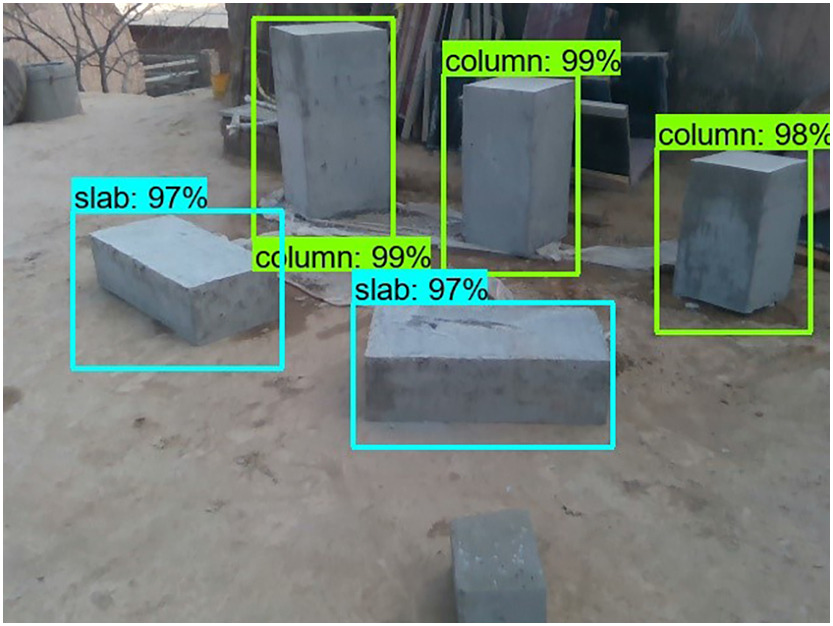
\includegraphics[width=0.6\linewidth]{object_reck.jpg}
    \caption{Ergebniss Foto des Objekterkennungsmodell von \cite{yong_object_2023}}
\end{figure}

Schliesslich untersucht die Arbeit von \cite{nasaMarkerReport} die Entwicklung und den Vergleich zweier Algorithmen zur Erkennung von 
Fiducial Markern. Ziel der Studie war es, mithilfe dieser Marker die Position und Orientierung des Roboters PUMA 560 präzise zu bestimmen. 
Die Marker bestehen aus einfachen geometrischen Formen wie Kreisen, Dreiecken und Quadraten. Die Arbeit vergleicht einen Algorithmus basierend 
auf Momentinvarianten mit einem zweiten, der eine diskrete Psi-S-Kurve verwendet. Letzterer erwies sich als überlegen und zeigte eine höhere 
Zuverlässigkeit bei der Marker-Erkennung. Diese Forschung liefert wertvolle Einblicke in die präzise Positionsbestimmung in Robotikanwendungen.

Um mit KI erfolgreich arbeiten zu können, ist ein Datensatz erforderlich, der bereits Bilder enthält, die korrekt markiert wurden. Solch ein Datensatz
wird genutzt, um ein KI-Modell zu trainieren. Leider konnten wir keinen Datensatz finden, der spezifisch auf unser Problem zugeschnitten ist. Ein eigener
Datensatz würde die Erstellung umfangreicher und zeitaufwendiger Annotationen erfordern, was den Rahmen dieses Projekts sprengen würde.

Zusätzlich müsste geprüft werden, ob die Kombination mit weiteren Sensoren wie Ultraschall- oder LiDAR-Kamerasystemen sinnvoll ist, um die Abstände sowie 
die Orientierung der Last und der Anschlagpunkte präzise zu bestimmen. Diese zusätzlichen Tests und Systeme wären jedoch mit Kosten verbunden und daher nicht praktikabel 
im Rahmen unserer aktuellen Ressourcen. Daher fokussieren wir uns darauf, die Position der Anschlagpunkte mithilfe von Fiducial Markern zu bestimmen.

\subsection{Fiducial Marker}
Fiducial Marker sind ein essenzielles Werkzeug in der modernen Bildverarbeitung und spielen eine 
zentrale Rolle in der räumlichen Orientierung und Positionsbestimmung. Insbesondere in Anwendungen 
wie der automatisierten Lastenhebung, wie sie von Ludwig System angestrebt wird, können Fiducial Marker 
helfen, Anschlagpunkte präzise zu lokalisieren.

Diese Marker, darunter Barcodes, QR-Codes oder speziell entwickelte AR-Marker, liefern visuelle 
Referenzen, die von Kamerasystemen erkannt und interpretiert werden können. Damit ermöglichen sie es, 
Objekte im Raum genau zu positionieren oder auszurichten.

In diesem Abschnitt untersuchen wir die Grundlagen von Fiducial Marker und beleuchten ihre spezifischen 
Einsatzmöglichkeiten in unserem Szenario, insbesondere im Kontext der automatisierten Ausrichtung von 
Anschlagpunkten auf der Traverse.

\subsubsection{Einführung Fiducial Marker}
Fiducial Marker sind quadratische Muster, die auf flachen Oberflächen aufgedruckt werden. 
Sie dienen als visuelle Referenzpunkte, die von Kamerasystemen erkannt und interpretiert 
werden können. Es gibt verschiedene Arten von Fiducial Marker, die je nach Anwendung 
unterschiedliche Eigenschaften und Einsatzmöglichkeiten bieten. 
Abbildung \ref{fig:marker_types} zeigt eine Auswahl solcher Marker.

\begin{figure}[H]
    \centering
    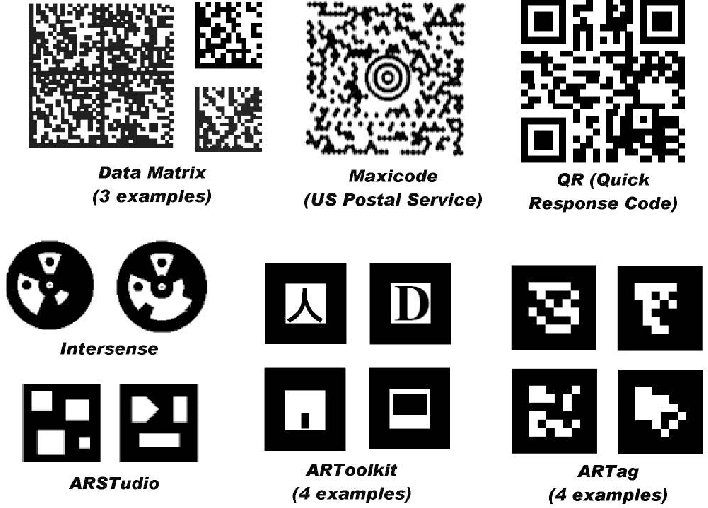
\includegraphics[width=0.7\linewidth]{graphics/marker_arten.png}
    \caption{Verschiedene Markerarten}
    \label{fig:marker_types}
\end{figure}

Grundsätzlich gilt: Je komplexer und grösser ein Marker ist, desto mehr Informationen können
darin gespeichert werden. Dabei muss jedoch der Informationsgehalt immer an die spezifischen 
Anforderungen der Anwendung angepasst werden, um eine optimale Balance zwischen Grösse, Lesbarkeit 
und Informationsdichte zu gewährleisten.

In der Robotik gehören AprilTags und AruCo-Marker zu den meistgenutzten Fiducial Marker. 
Ihre Beliebtheit basiert auf ihrer Robustheit und Effizienz bei der Lokalisierung in 
dreidimensionalen Räumen. Diese Marker wurden speziell entwickelt, um Verzerrungen und 
schwierige Lichtverhältnisse zu kompensieren und eine präzise Posenschätzung zu ermöglichen. 
Ihre Anwendung wird im weiteren Verlauf dieser Arbeit genauer beleuchtet, insbesondere im 
Kontext der automatisierten Lokalisierung von Anschlagpunkten.

\subsubsection {Wie AruCo und AprilTags erkannt werden}
AruCo-Marker und AprilTags sind quadratische Marker mit einem schwarzen Rand und einer binären Matrix, 
die spezifische Informationen wie die Marker ID encodiert. Der schwarze Rand erleichtert die schnelle Erkennung
der Marker in einem Bild, während die encodierte Matrix dazu dient, die ursprüngliche Orientierung
des Markers zu bestimmen. Die Grösse eines AruCo-Markers beeinflusst, wie viele Bits in der Matrix encodiert
werden können. Ein 4x4 AruCo-Marker besteht beispielsweise aus 16 Bits. Abbildung \ref{fig:sizes} zeigt 
Beispiele für verschiedene Grössen von AruCo-Markern. Der Marker unten rechts besteht aus einer 11x11-Matrix, 
was insgesamt 121 Bits ergibt.

\begin{figure}[H]
    \centering
    
\includegraphics[width=0.6\linewidth]{marker_sizes.png}
    \caption{Unterschiedliche Grössen von AruCo-Markern im Vergleich}
    \label{fig:sizes}
\end{figure}


Um AruCo-Marker detektieren zu können, müssen zunächst Parameter wie die Anzahl der Quadrate, die die Matrix encodieren,
sowie die tatsächliche Grösse in der gewünschten Einheit angegeben werden. Der Erkennungsprozess erfolgt dabei in zwei 
Hauptschritten. Im ersten Schritt wird das Bild auf potenzielle Marker-Kandidaten analysiert. Dabei werden die Konturen
im Bild segmentiert und die Quadratischen Konturen bleiben für die weitere Verarbeitung erhalten. 
Konturen, die zu klein, zu gross oder zu nah beieinander liegen werden ebenfalls verworfen.
Abbildung \ref{fig:segmentation} zeigt eine Visualisierung des Segmentationsprozesses und wie potenzielle
Marker-Kandidaten identifiziert werden.

\begin{figure}[H]
    \centering
    
\includegraphics[width=0.6\linewidth]{segmentation.png}
    \caption{Kontur Segmentation eines Bildes}
    \label{fig:segmentation}
\end{figure}

Nachdem die Kandidaten ausgewählt wurden, muss in einem zweiten Schritt geprüft werden, ob es sich tatsächlich um Marker handelt.
Dazu werden aus dem kalibrierten Bild die einzelnen Bits eines Markers extrahiert. Um schwarze von weissen Bits unterscheiden zu können,
wird das Bild zuvor binarisiert. Der Schwellenwert für die Binarisierung wird mithilfe von Otsu's Methode bestimmt.

Im Anschluss wird das Bild in Zellen aufgeteilt, wobei die Zellgrösse durch die Markergrösse und die Anzahl der Bits eines Markers festgelegt
wird. Nachdem das Bild in Zellen unterteilt wurde, wird die Anzahl der schwarzen und weissen Pixel in jeder Zelle gezählt, um festzustellen, 
ob es sich bei der Zelle um ein schwarzes oder weisses Bit handelt.

Abschliessend wird überprüft, ob die extrahierten Bits mit dem vorgegebenen Dictionary übereinstimmen, sodass die Marker eindeutig zugeordnet werden können.

AprilTags folgen einem ähnlichen Ansatz, sind jedoch für höhere Genauigkeit und Robustheit optimiert. Ein zentraler Unterschied ist, dass AprilTags für eine
bessere Fehlerkorrektur ausgelegt sind, was sie besonders für Anwendungen in der Robotik und Augmented Reality geeignet macht.



\subsubsection{Posenschätzung durch AR Marker}
Das Problem der Posenberechnung stammt aus dem Bereich der erweiterten 
Realität. Dabei wird eine Gleichung gelöst, die den Projektionsfehler 
zwischen den 2D-Bildpunkten und den 2D-Projektionen der 3D-Weltpunkte minimiert. 
Das Lösen dieser Gleichung liefert einen Rotations- und Translationsvektor, der 
die Position und Orientierung der Kamera im Koordinatensystem beschreibt. 
Abbildung \ref{fig:pose} illustriert diesen Zusammenhang.

\begin{figure}[H]
    \centering
    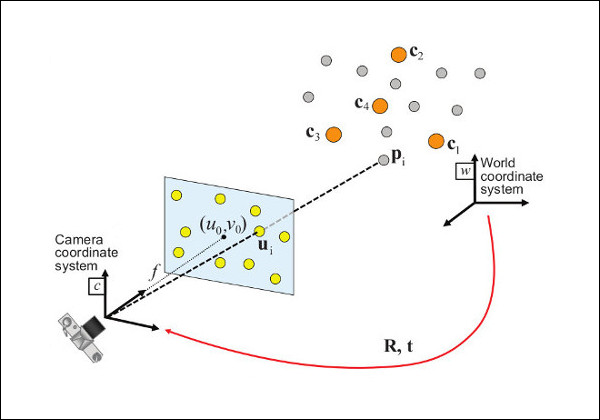
\includegraphics[width=0.4\linewidth]{graphics/pose.png}
    \caption{Posenschätzung}
    \label{fig:pose}
\end{figure}

Laut \cite{pose} braucht es dazu folgende Komponenten: die intrinsischen Parameter 
der Kamera \( K \) und die Projektionsmatrix \( \Pi \). Die intrinsischen Parameter 
können bereits vorher durch die Kalibrierung der Kamera berechnet werden. Die Kalibrierung 
wird mit OpenCV-Methoden durchgeführt, wie in \cite{zhang} und \cite{bradski} detailliert 
beschrieben.

Mithilfe der beiden Matrizen lässt sich eine Gleichung aufstellen, die \( N \) Punkte 
in der 3D-Welt auf 2D-Bildpunkte projiziert. Dabei entstehen die Rotationsmatrix und der 
Translationsvektor, die in der Transformationsmatrix \(\mathbf{T}^c_{w}\) enthalten sind.
Mit der Schätzung dieser Matrix können Weltkoordinaten in Kamerakoordinaten transformiert 
werden.

Gleichung um Weltkoordinaten im Bild zu projizieren:
\[
\begin{bmatrix}
u \\ 
v \\ 
1
\end{bmatrix}
=
\mathbf{A} \mathbf{\Pi} \mathbf{T}^c_{w}
\begin{bmatrix}
X_w \\ 
Y_w \\ 
Z_w \\ 
1
\end{bmatrix}
\]

\[
\begin{bmatrix}
u \\ 
v \\ 
1
\end{bmatrix}
=
\begin{bmatrix}
f_x & 0   & c_x & 0 \\ 
0   & f_y & c_y & 0 \\ 
0   & 0   & 1   & 0
\end{bmatrix}
\begin{bmatrix}
1 & 0 & 0 & 0 \\ 
0 & 1 & 0 & 0 \\ 
0 & 0 & 1 & 0
\end{bmatrix}
\begin{bmatrix}
r_{11} & r_{12} & r_{13} & t_x \\ 
r_{21} & r_{22} & r_{23} & t_y \\ 
r_{31} & r_{32} & r_{33} & t_z \\ 
0      & 0      & 0      & 1
\end{bmatrix}
\begin{bmatrix}
X_w \\ 
Y_w \\ 
Z_w \\ 
1
\end{bmatrix}
\]

Gleichung um Weltkoordinaten in Kamerakoordinaten zu transformieren:

\[
\begin{bmatrix}
X_c \\ 
Y_c \\ 
Z_c \\ 
1
\end{bmatrix}
=
\mathbf{T}^c_{w}
\begin{bmatrix}
X_w \\ 
Y_w \\ 
Z_w \\ 
1
\end{bmatrix}
\]

\[
\begin{bmatrix}
X_c \\ 
Y_c \\ 
Z_c \\ 
1
\end{bmatrix}
=
\begin{bmatrix}
r_{11} & r_{12} & r_{13} & t_x \\
r_{21} & r_{22} & r_{23} & t_y \\
r_{31} & r_{32} & r_{33} & t_z \\
0 & 0 & 0 & 1
\end{bmatrix}
\begin{bmatrix}
X_w \\ 
Y_w \\ 
Z_w \\ 
1
\end{bmatrix}
\]

\subsubsection{Probleme mit Fiducial Marker}
Mithilfe von Fiducial Marker können wir Anschlagpunkte erkennen und dessen Position bestimmen.
Zusätzlich können wir mit deren Hilfe ausrechnen wie sich die Traverse Positionieren musss, damit
sich über den den Anschlagspunkten befindent.

Allerdings stellen Fiducial Marker  keine perfekte Lösung dar, um Anschlagpunkte zuverlässig zu lokalisieren. 
Sie sind besonders empfindlich gegenüber äusseren Einflüssen. Bereits geringe Verschmutzungen, 
wie etwa Schmutz oder Staub auf den Kanten, können die Erkennung erheblich beeinträchtigen 
oder sogar vollständig verhindern.

Darüber hinaus sind Fiducial Marker anfällig für ungünstige Lichtverhältnisse. Blendung, Schatten 
oder Reflexionen können die Erkennungsrate deutlich verringern, insbesondere in Aussenbereichen 
oder bei wechselnden Lichtbedingungen. Auch der Erkennungsbereich der Marker ist begrenzt: Marker 
müssen sich in einem bestimmten Abstand und Winkel zur Kamera befinden um erkannt zu werden.

Grössere Marker können zwar leichter erkannt werden, bringen jedoch eigene Herausforderungen mit sich. 
insbesondere wenn auf der Last nicht genügend Platz für die Anbringung verfügbar ist. Zudem nutzen 
sich Marker durch äussere Einflüsse, wie Witterung oder mechanische Belastung, schnell ab. Um die 
Erkennung dauerhaft zu gewährleisten, müssen sie regelmässig ersetzt oder neu angebracht werden.


\clearpage
\subsection{Kameras}
Um die Anschlagpunkte zuverlässig erkennen zu können, sind geeignete Kamerasysteme
erforderlich. Um zu verstehen, warum bestimmte Schritte, wie beispielsweise die 
Kalibrierung der Kamera, notwendig sind und warum es zu Ungenauigkeiten bei den 
Berechnungen zur Positionierung der Traverse kommen kann, betrachten wir in diesem 
Abschnitt die Funktionsweise und Eigenschaften von Kamerasystemen genauer.

\subsubsection{Kameraeigenschaften}
Eine Kamera kann ein Bild generieren, das insgesamt \( L \) Pixel in 
der Länge und \( H \) Pixel in der Höhe besitzt. \( L \) und \( H \) 
beschreiben hierbei die Auflösung der Kamera. Die Auflösung ist ein 
wichtiger Faktor, da sie bestimmt, wie viele Details in einem Bild 
sichtbar sind. Höhere Auflösungen ermöglichen genauere Berechnungen, 
erfordern jedoch auch mehr Rechenleistung für die Verarbeitung der 
Bilder.

Das FOV (Field of View) einer Kamera beschreibt den Bereich der Szene,
den die Kamera sehen oder aufnehmen kann. Es ist ein grundlegender 
Parameter, der angibt, wie viel von der Umgebung eine Kamera in einem 
Bild oder Video erfassen kann. Je höher das FOV, desto grösser ist 
jedoch die Verzerrung, die im Bild entsteht.
Abbildung \ref{fig:fisheye} zeigt, wie eine starke Verzerrung aussieht,
die typischerweise bei Weitwinkel- oder Fisheye-Objektiven auftritt.

\begin{figure}[H]
    \centering
    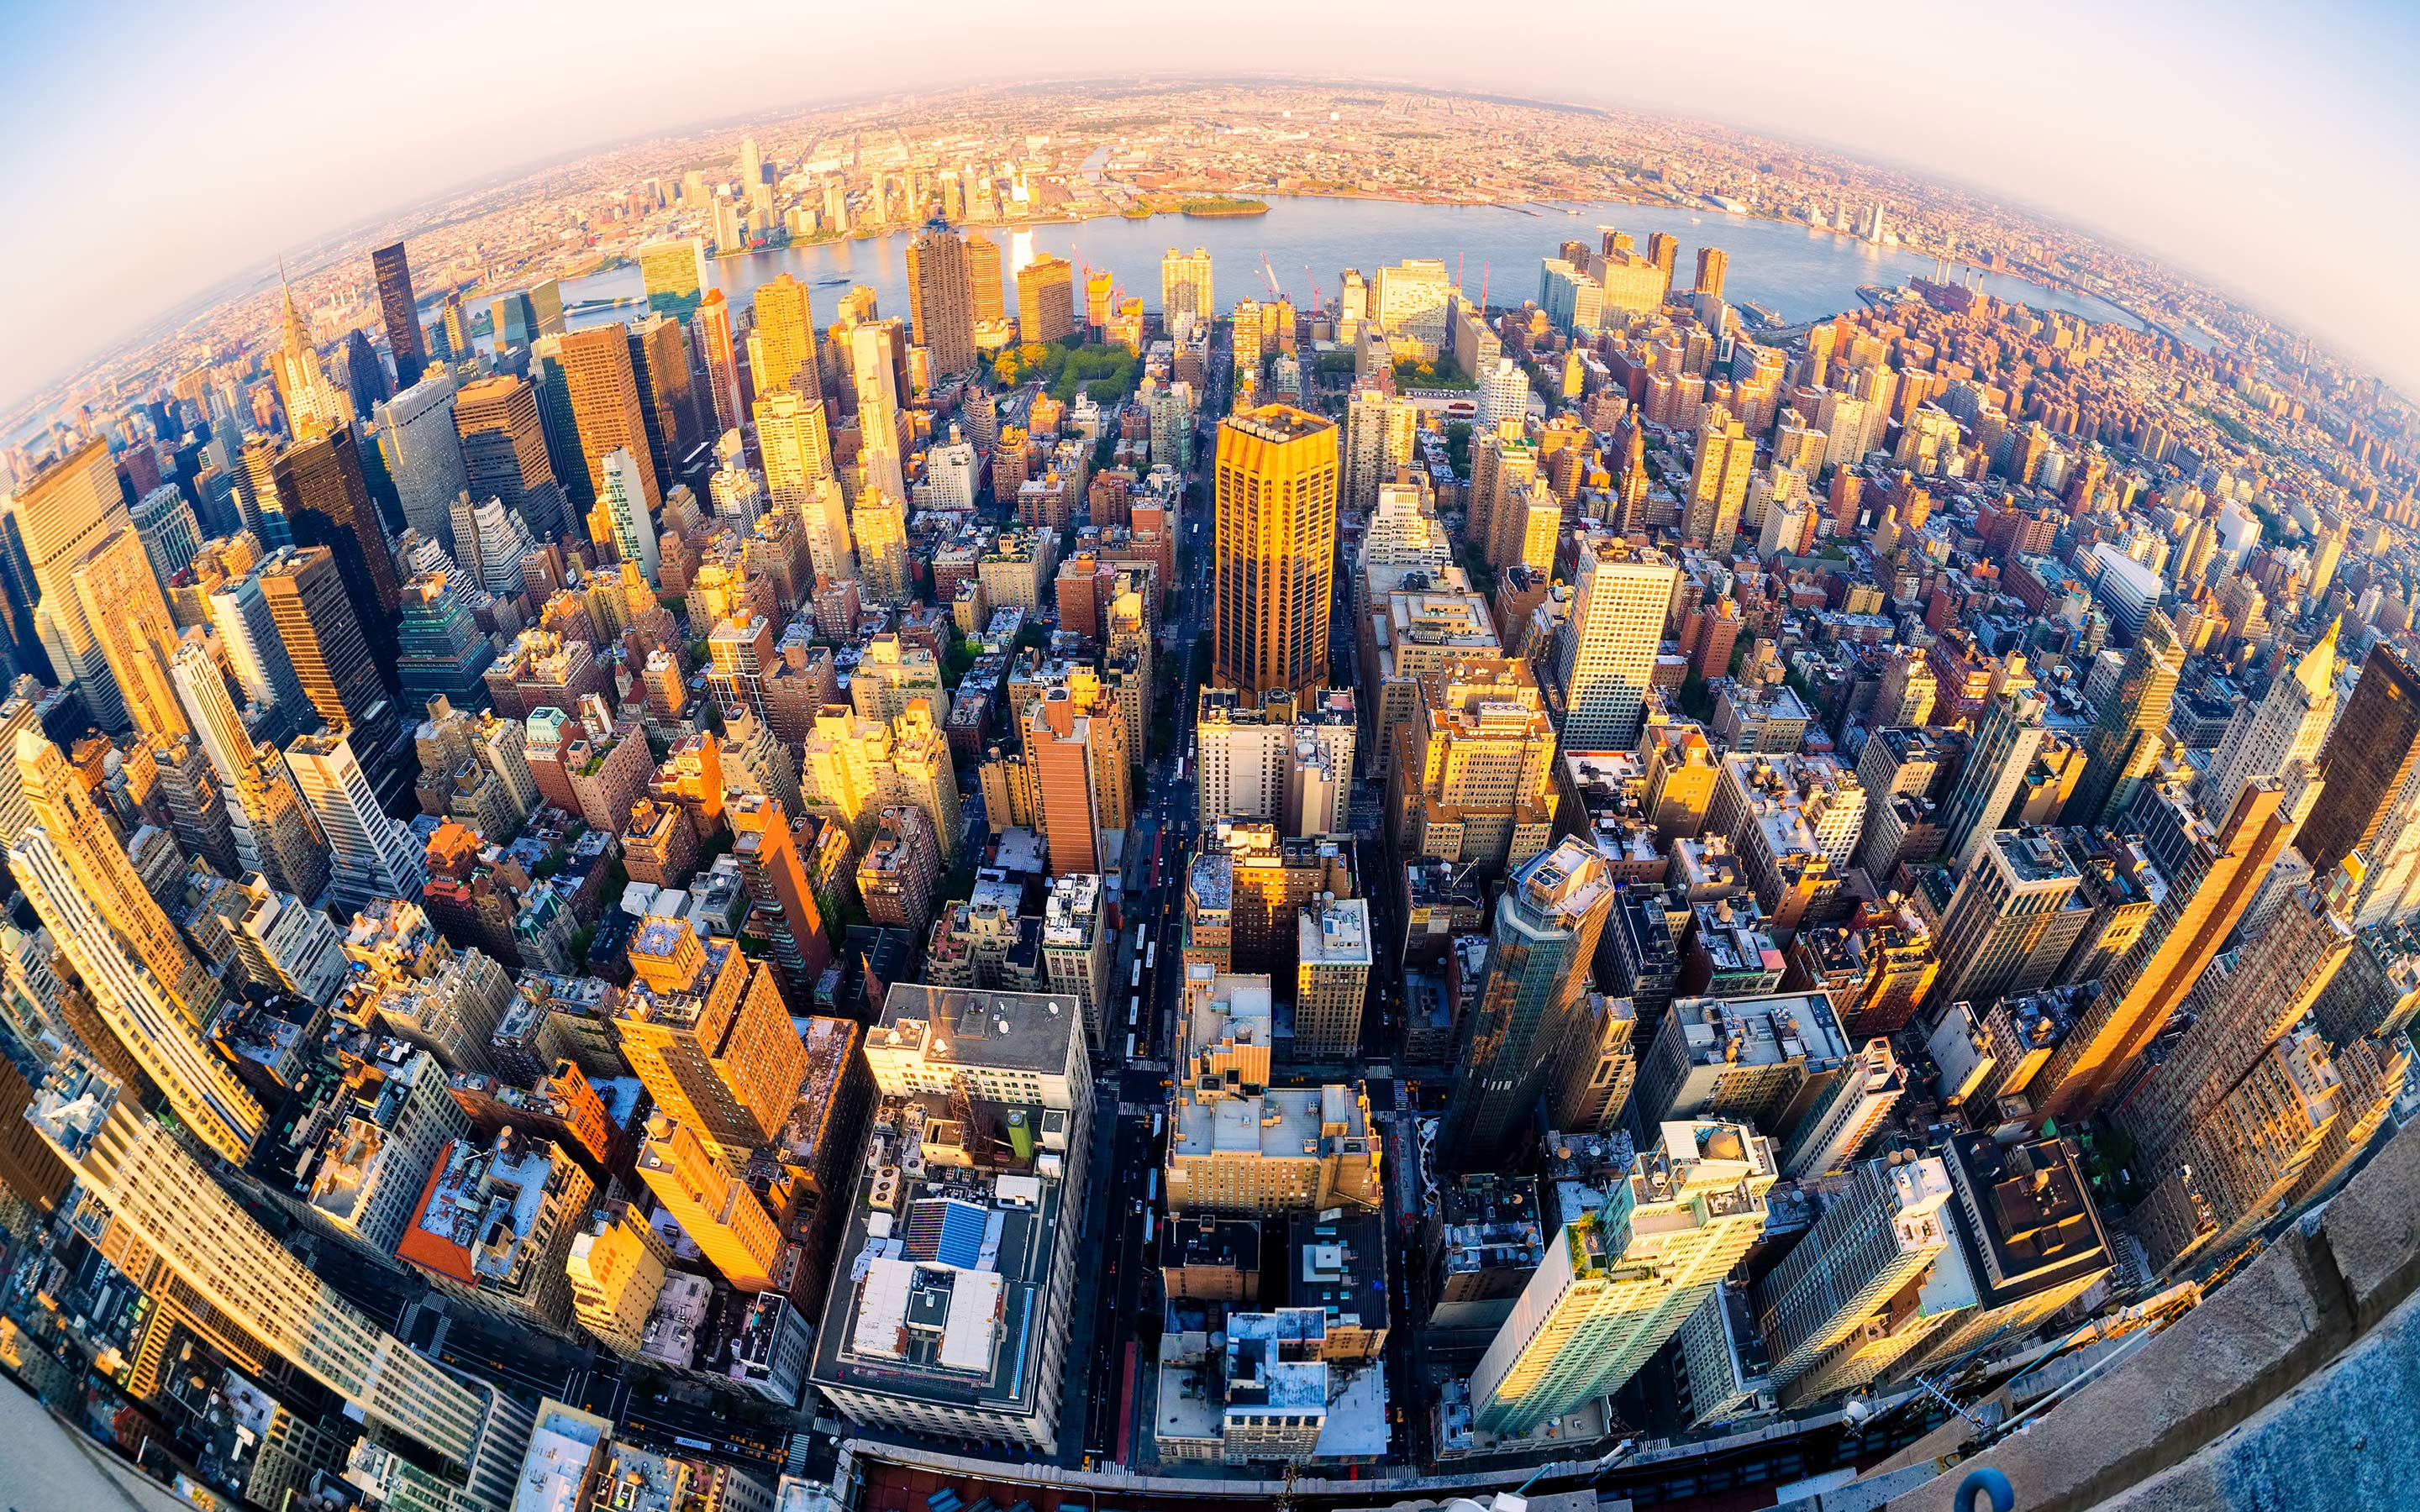
\includegraphics[width=0.5\linewidth]{graphics/fisheye.jpg}
    \caption{Beispielfoto einer starken Verzerrung}
    \label{fig:fisheye}
\end{figure}

Neben Auflösung und FOV gibt es weitere wichtige Eigenschaften, die 
bei der Auswahl und Nutzung einer Kamera berücksichtigt werden sollten:

\begin{itemize}
    \item \textbf{Bildrate (Frame Rate):} Gibt an, wie viele Bilder pro Sekunde aufgenommen werden können.
    \item \textbf{Fokus und Tiefenschärfe:} Der Fokusbereich beeinflusst, welche Bereiche des Bildes scharf dargestellt werden.
\end{itemize}


\subsubsection{Intrinsische Kalibrierung}
Verzerrungen, insbesondere an den Kanten eines Bildes, können zu Rechenfehlern 
bei der Positionierung der Traverse führen. Verzerrungen entstehen durch optische 
Abweichungen der Linse und sind besonders bei hohen FOV-Werten ausgeprägt. 
Zudem können sie die Erkennung der Anschlagpunkte erschweren, da die Form und 
Lage der Marker falsch interpretiert werden können.

Es gibt zwei Hauptarten von Verzerrungen bei Kameralinsen: die radiale und die tangentiale Verzerrung.
Die radiale Verzerrung führt dazu, dass eigentlich gerade Linien gekrümmt erscheinen. Abbildung 
\ref{fig:distortion} verdeutlicht die Auswirkung der radiale Verzerrung, bei der gerade Linien gekrümmt
dargestellt werden.

\begin{figure}[H]
    \centering
    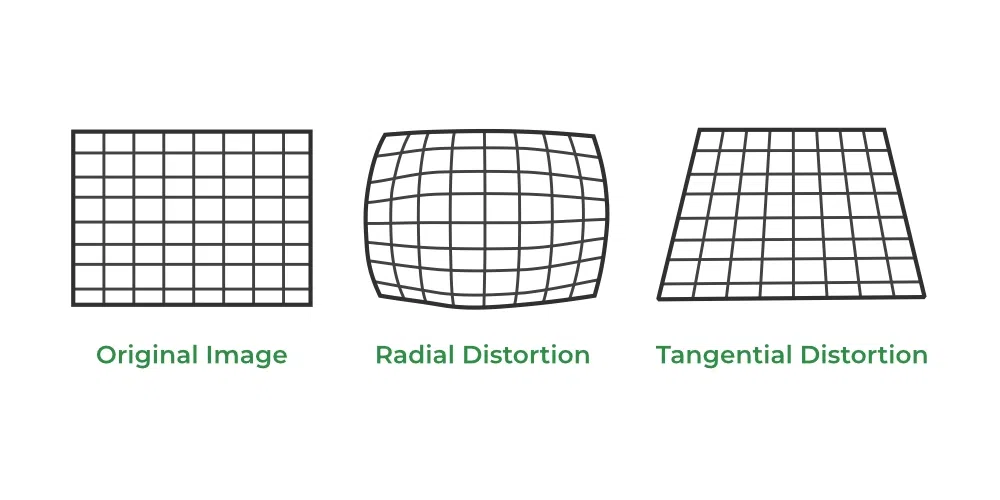
\includegraphics[width=\linewidth]{distortion.png}
    \caption{Beispiele von Verzerrungen}
    \label{fig:distortion}
\end{figure}

Die tangentiale Verzerrung entsteht, wenn die Kameralinse nicht perfekt parallel zur Bildebene ausgerichtet
ist. Dies führt dazu, dass bestimmte Bereiche des Bildes näher erscheinen als andere, wodurch eine ungleichmässige
Darstellung entsteht. 

Die radiale Verzerrung lässt sich mit folgender Formel berechnen:

\[
x_\text{distorted} = x(1 + k_1r^2 + k_2r^4 + k_3r^6) \quad
y_\text{distorted} = y(1 + k_1r^2 + k_2r^4 + k_3r^6)
\]

Die Formel zur Berechnung der tangentialen Verzerrung lautet:

\[
x_\text{distorted} = x + \left[ 2p_1xy + p_2(r^2 + 2x^2) \right]
y_\text{distorted} = y + \left[ p_1(r^2 + 2y^2) + 2p_2xy \right]
\]

Das \(r\) ist hierbei für den euklidischen Abstand, den ein Pixel mit Koordinaten \((x, y)\) zum Bildzentrum hat.
Zusammengefasst muss man also die Verzerrungskoeffizienten k1, k2, p1, p2 und k3 finden.

\[
Verzerrungskoeffizienten = (k1, k2, p1, p2, k3)
\]

Zusätzlich zu den Verzerrungskoeffizienten werden auch die intrinsischen Parameter der Kamera benötigt. Diese können 
mithilfe eines vorgegebenen Kalibrierungsmusters berechnet werden. Dabei werden bekannte Punkte des Musters verwendet,
deren tatsächliche Positionen in Weltkoordinaten bekannt sind. Anschliessend werden diese Punkte auf die Bildkoordinaten
projiziert. Die Kalibrierung minimiert iterativ den Reprojektion-Fehler, der die Differenz zwischen den projizierten 
Punkten und den gemessenen Bildpunkten darstellt.

\[
K =
\begin{bmatrix}
f_x & 0 & c_x \\
0 & f_y & c_y \\
0 & 0 & 1
\end{bmatrix}
\]

Die Kamerakalibrierung umfasst die Korrektur von Verzerrungen sowie die Bestimmung der 
intrinsischen Parameter der Kamera, wie:

\begin{itemize}
    \item \textbf{Brennweite} (\( f_x, f_y \)): Gibt an, wie stark die Linse das Licht bündelt.
    \item \textbf{Hauptpunkt} (\( c_x, c_y \)): Die Koordinaten des optischen Zentrums auf dem Bildsensor.
    \item \textbf{Verzerrungskoeffizienten}: Parameter, die die Stärke der Verzerrungen beschreiben.
\end{itemize}


Um eine Kamera zu kalibrieren, werden mehrere Fotos eines regelmässigen Musters 
benötigt. Die Bilder sollten aus verschiedenen Distanzen und Blickwinkeln aufgenommen werden,
um eine möglichst breite Datenbasis zu schaffen. Dabei ist es wichtig die Kamera zu bewegen, während
das Muster fest positioniert bleibt. Abbildung \ref{fig:corrected} zeigt die Korrektur von Verzerrungen
anhand eines Kalibrierungsmusters, wobei die Verzerrung vor und nach der Kalibrierung sichtbar ist.

\begin{figure}[H]
    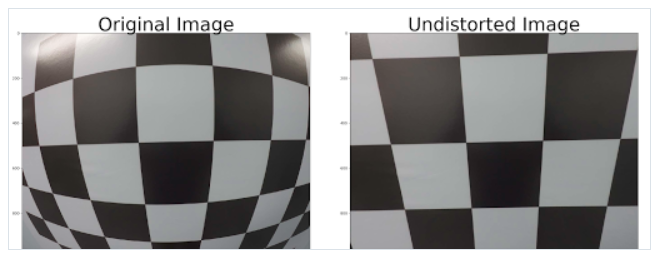
\includegraphics[width=\linewidth]{corrected.png}
    \caption{Muster vor und nach der Kalibrierung}
    \label{fig:corrected}
\end{figure}

Die Dokumentation von OpenCV \cite{opencv_calibration_tutorial} liefert praktische 
Beispiele und erklärt detailliert, wie die Kalibrierung implementiert werden 
kann.


\subsection{Benutzte Frameworks}
OpenCV ist eine populäre Open-Source-Bibliothek für verschiedene Bildverarbeitungssoftware.
Open Source bedeutet, dass die Funktionen für jeden frei verfügbar sind. OpenCV bietet 
umfangreiche Funktionen, um AruCo-Marker zu erkennen und eine Kamerakalibration durchzuführen.
Weitere Informationen zu OpenCV finden sich auf der offiziellen Webseite unter opencv.org.

Allerdings unterstützt OpenCV keine Erkennung von AprilTags. Um diese Aufgabe zu erfüllen, verwenden 
wir stattdessen eine spezielle Ressource, die im GitHub-Repository für AprilTags bereitgestellt 
wird \cite{apriltag_github}. Dieses Repository basiert auf drei wissenschaftlichen Arbeiten 
\cite{olson2011tags} \cite{wang2016iros} \cite{krogius2019iros} und bietet eine effiziente 
und robuste Lösung zur Erkennung von AprilTags. Die Software wird unter der BSD 2-Clause License 
veröffentlicht, die eine freie Nutzung, Modifikation und Weiterverteilung unter bestimmten Bedingungen 
erlaubt. Weitere Details zur Lizenz können direkt im Repository nachgelesen werden.
\section{Konzept}

Ludwig Systems benötigt eine Lösung, welche von der Traverse aus die Ist-Koordinaten, die Rotation und Neigung der Last ausgibt. Das Konzept soll dieses Ziel um in der Zukunft die Traverse automatisch bewegen zu können. Des Weiteren soll das Konzept sicherstellen, dass die Genauigkeiten ,welche vom Kunden gegeben wurde, eingehalten werden können.

\subsection{Konzept 1: Objekterkennung durch Machine Learning}

\subsection{Konzept 2:  Posenschätzung durch AR Marker}

\subsection{Evaluation Konzepte}

\subsection{Intrinsische Kalibrierung der Kamera}
(Erklärung wie die Kalibrierung funktioniert )

\subsection{Lokalisierung Last}
(Erklärung wie die Lokalisierung mithilfe von Marker funktionieren sollte.)
\subsubsection{Marker Anordnung}
(Erklärung Anordnung und wieso)
\subsubsection{Marker Grösse}
(Erklärung der Rechnung für Marker Grösse)
\subsubsection{Mittelpunkt-Berechnung der Marker Anordnung}
(Erklärung der Rechnung um vom Diamand-Marker-Muster auf die Mitte) 

\subsection{Kamera Spezifikationen}
(Erklärung welche Kamera Eigenschaften gebraucht werden und wieso wir diese brauchen.)
\subsubsection{Kamera Position}
(Erklärung wo Kameras Positioniert sind und Rechnung von horizontale FOV)
\subsubsection{Kamera Eigenschaften}
(Erklärung der Rechnung horizontale Bildauflösung und auflistung aller Eigenschaften ausgehend der Marker Grösse.)

\section{Implementierung}

In diesem Kapitel wird die Implementierung erläutert vom Marker Konzept. 
Es werden die Umsetzung der Intrinsischen Kamera Kalibrierung beschrieben und die zwei Implementierungen, eine mit ArUco Marker der andere mit AprilTags, erläutert und evaluiert.
Zusätzlich werden die Umsetzungen der Posenschätzung und der Mittelpunkt-Berechnung beschrieben.

\subsection{Intrinsische Kamera Kalibrierung}

Um eine genaue Posenschätzung durchführen zu können, braucht man erst die Kamera Matrix und die Verzerrungs-Koeffizienten. 
Die Kamera Matrix ist eine 3x3 Matrix, welches die Fokus Länge und optische Zentren besitzt. 
Die Kamera Matrix würde so aussehen:
\begin{bmatrix}
fx & 0 & cx \\ 
0 & fy & cy \\ 
0 & 0  & 1 
\end{bmatrix}

Um eine Kalibrirung durchzuführen, braucht es Test-Fotos eines Kalibrierungs-Muster. 
Die Abbildung\ref{fig:Pattern} zeigt ein 9x6 Schachbrett-Muster, welches für diese Implementierung benutzt worden ist, um die Kalibrierung durchzuführen.
Für genauere Kalibrierungs-Werte sollten mindestens 10 Fotos vom Schachbrett-Muster gemacht werden\cite{noauthor_opencv_nodate-2}


\begin{figure}[H]
    \centering
    
\includegraphics[width=\linewidth]{graphics/pattern.png}
    \caption{Ein 9x6 Schachbrett-Muster, welches für Kamera-Kalibrierung benutzt wird}
    \label{fig:Pattern}
\end{figure}

\begin{lstlisting}[language=Python, caption=Bilder laden für Kalibrierung]
    image_files = glob.glob('./imgs/*.jpg')
    images = [cv2.imread(file) for file in image_files]
\end{lstlisting}

Alle Bilder innerhalb des "./imgs" Ordner werden geladen und als cv image abgespeichert. 

\begin{lstlisting}[language=Python, caption=Methode um Schachbrett Ecken zu finden]
    def find_chessboard_corners(images, pattern_size):
    obj_points = []
    img_points = []

    # Prepare the 3D points of the chessboard corners (0,0,0), (1,0,0), (2,0,0) ..., (6,5,0)
    objp = np.zeros((pattern_size[0] * pattern_size[1], 3), np.float32)
    objp[:, :2] = np.mgrid[0:pattern_size[0], 0:pattern_size[1]].T.reshape(-1, 2)

    for img in images:
        gray = cv2.cvtColor(img, cv2.COLOR_BGR2GRAY)
        ret, corners = cv2.findChessboardCorners(gray, pattern_size, None)

        if ret:
            obj_points.append(objp)
            img_points.append(corners)

    return obj_points, img_points
\end{lstlisting}

In der Methode find_chessboard_corners werden die Object Points und image Points ausgegeben. Object Points sind die 3D Punkte der Schachbrett-Muster Ecken.
Dann wird jedes Bild zu einem Graustufen-Bild umgewandelt, da dass SchabrettMuster Schwarz-Weiss ist, braucht es die RGB Werte nicht. 
Durch die findChessboardCorners von opencv erhält man alle image points, also die Ecken des Schachbrett-Musters, und ret. 
Ret besagt ob ein Schabrett-Muster gefunden worden ist und falls das der Fall ist werden die Object Points und Image Points erweitert.

\begin{lstlisting}[language=Python, caption=Methode um Kamera zu kalibrieren]
    def calibrate_camera(obj_points, img_points, img_size):
        ret, mtx, dist, rvecs, tvecs = cv2.calibrateCamera(obj_points, img_points, img_size, None, None)
        return ret, mtx, dist, rvecs, tvecs
\end{lstlisting}

Die Object Points und Image Points können dann in die calibrateCamera Methode von opencv eingefügt werden, um die Kamera Matrix und die Verzerrungs-Koeffizienten zu bekommen.

\begin{lstlisting}[language=Python, caption=Speicherung der Kalibrierungs-Daten in einer Datei]
    # Save parameters to a file
    cv_file = cv2.FileStorage(save_path, cv2.FILE_STORAGE_WRITE)
    cv_file.write('K', camera_matrix)
    cv_file.write('D', dist_coeffs)
    cv_file.release()
\end{lstlisting}

Zuletzt werden die Kamera Matrix und Verzerrungs Koeffizienten in eine Datei gespeichert, so dass diese bei einem neuen Start wieder verwendet werden können ohne kalibrieren zu müssen.

Falls sich der Fokus der Kamera oder eine andere Kamera Eigenschaft verändert wird, muss diese Kalibrierung neu gemacht werden, um so die neue Kalibrierungs Datei benutzen zu können.

\subsection{Lokalisierung der Last}

\subsubsection{Implementierung: ArUco}

\begin{lstlisting}[language=Python, caption=ID und Ecken eines ArUco Markers erkennen]
    marker_dict = aruco.getPredefinedDictionary(cv.aruco.DICT_4X4_1000)
    param_markers = cv.aruco.DetectorParameters()
    detector = cv.aruco.ArucoDetector(marker_dict, param_markers)
    marker_corners, marker_IDs, reject = detector.detectMarkers(image)
    
    total_markers = range(0, marker_IDs.size)
\end{lstlisting}

Um ein ArUco Marker erkennen zu können muss man erst die Dictionary des Ausgewählten Markers definieren. 
In dieser Implementierung ist es die DICT_4X4_1000.
Danach muss ein Detector initialisiert werden und damit kann man in einem Bild alle Marker Ecken und IDs bekommen.
Durch diese kann man dann durch iterieren um für jeden gefundenen Marker eine Posenschätzung durchzuführen.

\subsubsection{Implementierung: AprilTag}

\subsubsection{Umsetzung Posenschätzung der Marker}
(Erklärung der Umsetzung der Posenschätzung sowie die ersten Resultate zeigen und evaluieren welche besser ist)

\subsubsection{Umsetzung der Mittelpunkt-Berechnung}

Da man nicht die Koordinaten der Marker braucht, sondern die des Anschlagspunkts, muss man eine Mittelpunkt-Berechnung durchführen wie im Kapitel \ref{sec:middlePoint} beschrieben.

\begin{lstlisting}[language=Python, caption=ID und Ecken eines ArUco Markers erkennen]
    pointTranslations = [np.array([6.3,0,0]),np.array([0,-6.3,0]),np.array([-6.3,0,0]),np.array([0,6.3,0])]

    rVec, tVec, _ = my_estimatePoseSingleMarkers(corners, markerSize, mtx, dist)
    tVec = np.array(tVec)
    rVec = np.array(rVec)

    rmtx,_ = cv2.Rodrigues(rVec[i][0])
    translate = np.matmul(rmtx, pointTranslations[ids%4])
    point = np.add(tVec[i][0].flatten(),translate)
\end{lstlisting}

Man führt zuerst die Posenschätzung aus um die Translations und Rotations Vektoren zu bekommen.
Mit der Rodrigues Methode kann man den Rotations Vektor zu einer Rotations Matrix umwandeln.
Dann muss man die Translation zur Mitte zusammen mit der Rotationsmatrix zusammenrechnen um so eine richtig rotierte Translation zur Mitte zu bekommen.
Welche Translation benutzt werden muss wird, wie im Kapitel \ref{sec:middlePoint} beschrieben, durch die ID des Markers Modulo 4 definiert, da es 4 pro Anschlagspunkt gibt.

Schlussendlich wird auf die Translations Vektor vom Marker die Tranlation zur Mitte addiert und so bekommt man den Mittelpunkt der Anordnung.




\section{Evaluation und Diskussion}

\subsection{Testumgebung}

Um zu testen ob die Implementierung die Anforderungen erfüllen kann, mussten Test-bilder geschossen werden.

So dass die Test-Bilder genau sind und aus den resultierenden Posenschätzungen die Genauigkeit bestummen werden kann, wurde eine Testumgebung aufgebaut.

\begin{figure}[H]
    \centering
    \begin{subfigure}[h]{0.5\textwidth}
        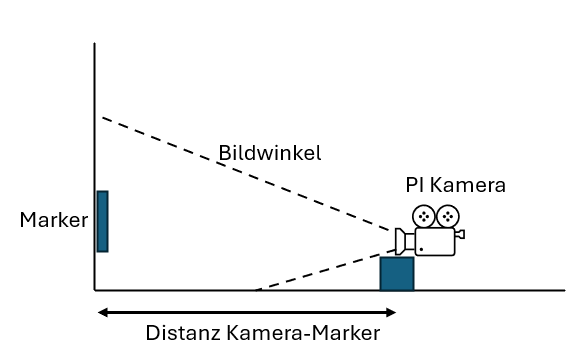
\includegraphics[width=0.5\textwidth]{graphics/Skizze_TestUmgebung.PNG}\hfill%
        \caption{Skizze der Testumgebung}
        \label{fig:SkizzeTestumgebung}
    \end{subfigure}
    \quad
    \begin{subfigure}[h]{0.5\textwidth}
        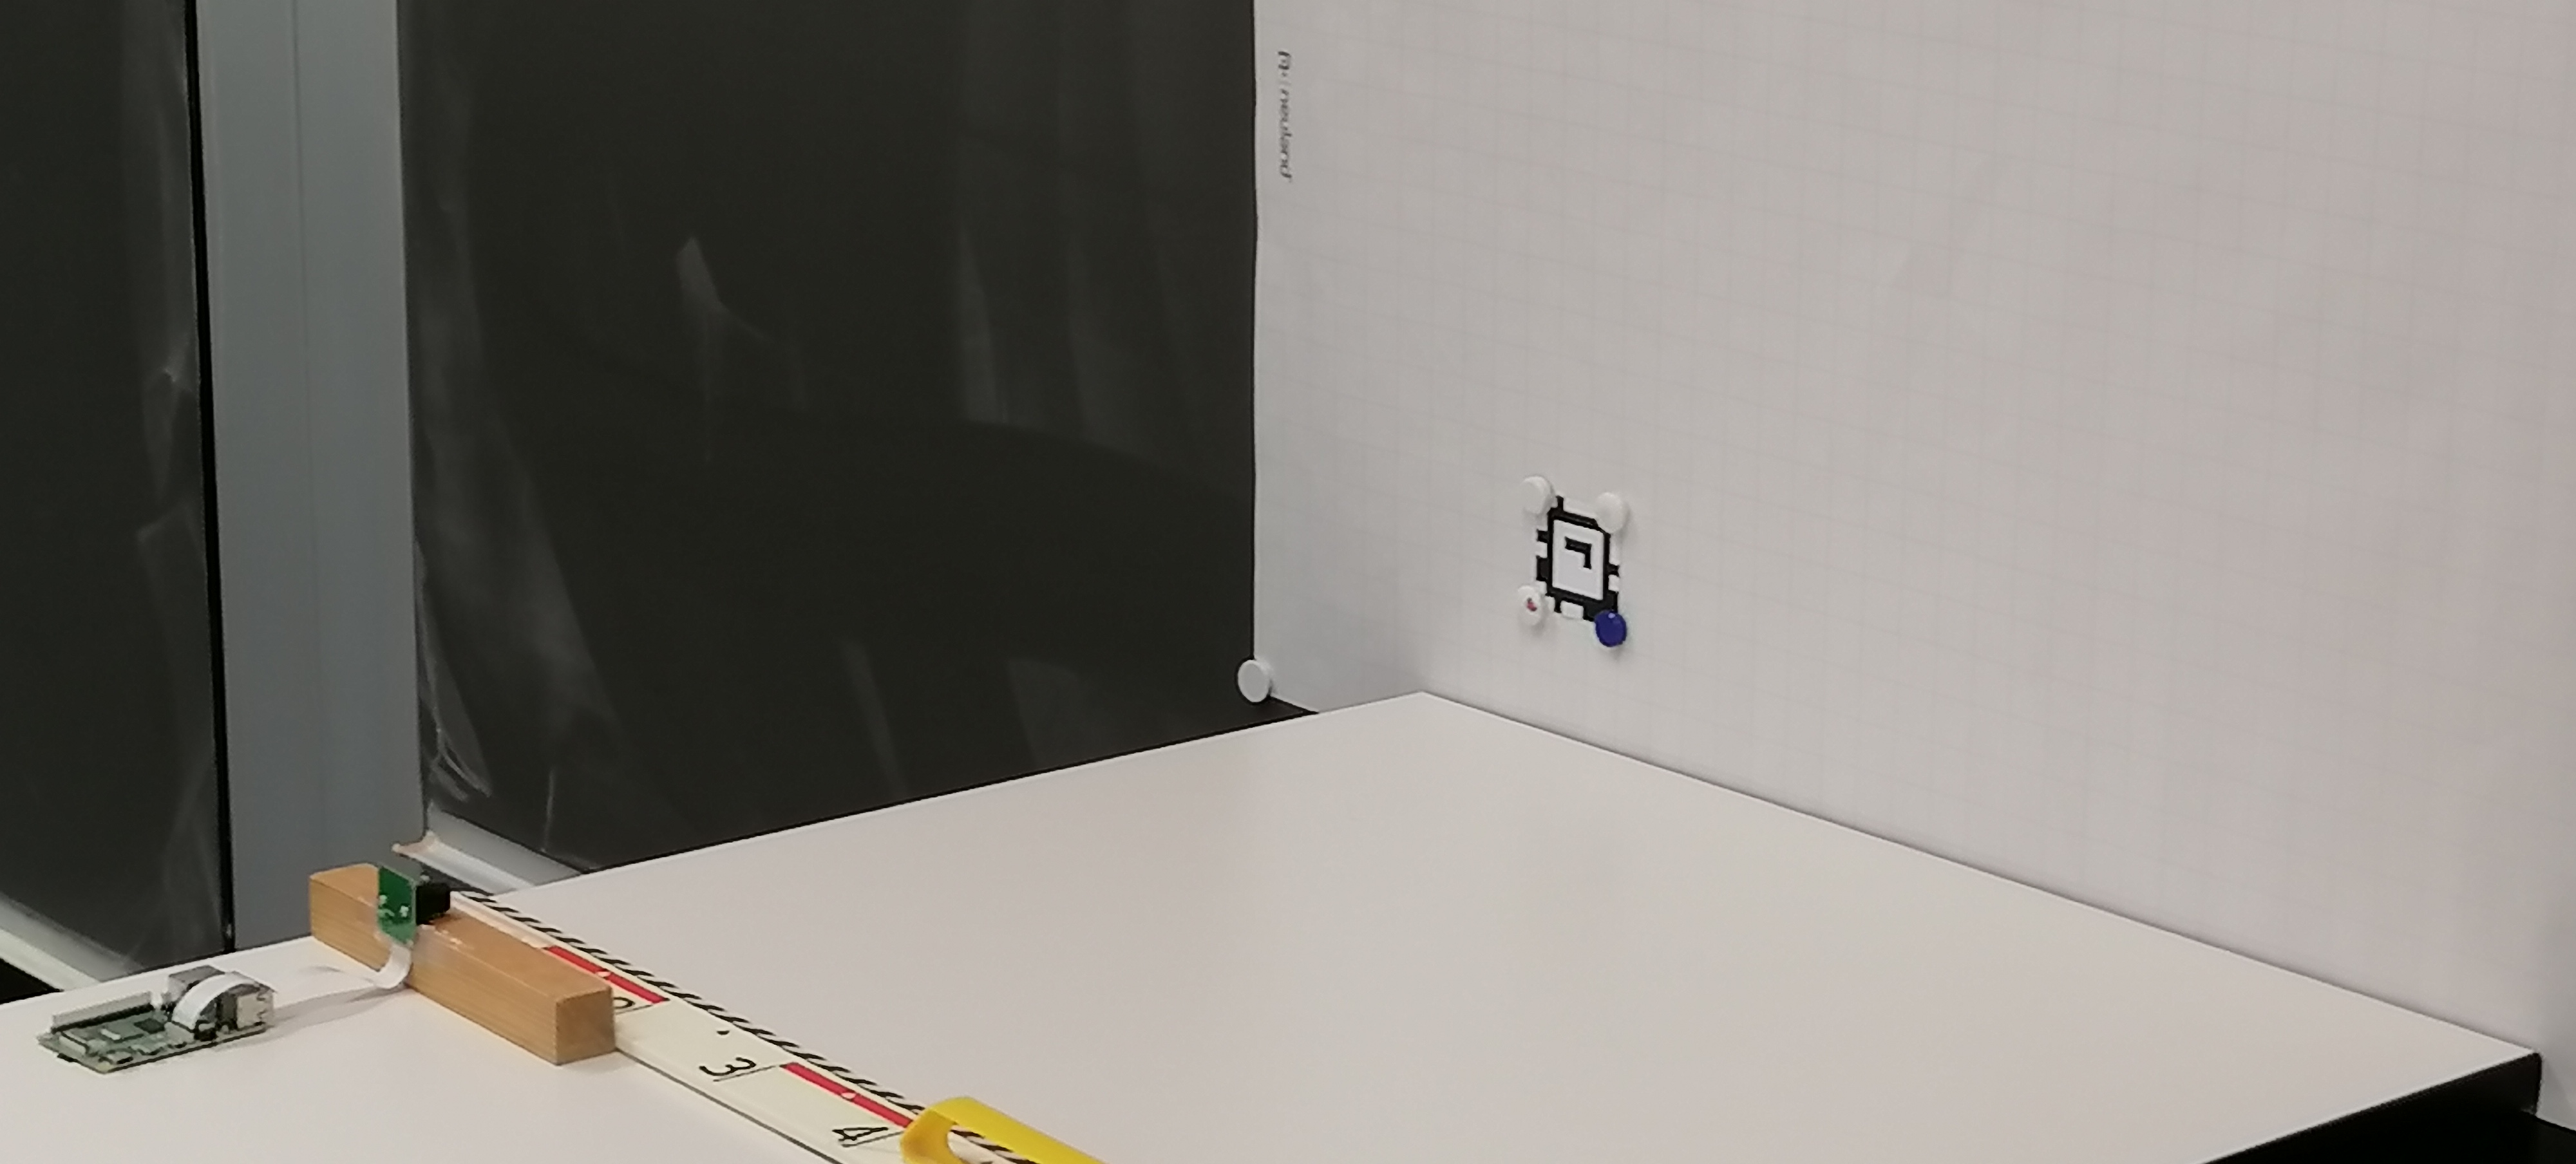
\includegraphics[width=0.5\textwidth]{graphics/TestUmgebung.jpg}\hfill%
        \caption{Implementierung der Testumgebung}
        \label{fig:Testumgebung}
    \end{subfigure}
    \caption{Beschreibung der Testumgebung}
\end{figure}

Die Abbildung \ref{fig:SkizzeTestumgebung} beschreibt wie die Testumgebung aufgebaut werden sollte.
Die Kamera sollte auf einem Objekt stabilisiert werden, um ein stabileres Bild zu bekommen und dass die Kamera höher gelagert ist und so mehr sehen kann.

Die Marker sollten auf einer Wand befestigt werden. 
Um einen fairen Vergleich zwischen Apriltag und ArUco machen zu können, wurden beide für die Posenschätzung nebeneinander auf einem Bild Fotografiert.
Dies stellt sicher dass beide Marker gleich entfernt sind und kleine Verschiebungen beide beinträchtigen.

Die Test-Fotos wurden von den Distanzen 75 cm, 100 cm, 150 cm und 200cm.
75 cm und 200 cm sind jeweils die Mindesthöhe und die Maximalhöhe, bei welcher das System funktionieren sollte.
100 cm und 150 cm wurden gewählt, um sehen wie die Ungenauigkeit sich über die Distanzen entwickelt.

Bei der Abbildung \ref{fig:Testumgebung} wird gezeigt wie die Implementierung der Skizze aussieht. 
Es wurde die Raspberry Pi Kamera Model B Rev 2.0 als Test-Kamera benutzt, welche auf einen Holzblock stabilisiert wurde.
Mit einem 1 Meter Lineal wurde sichergestellt, dass der Holzblock und damit die Kamera relativ zu den Marker gerade war.
Mit einem Messgerät wurde die Distanz vom Marker zur Kamera gemessen. 
Dabei musste noch die Länge des Objektives mitberechnet werden, da das Bild vom Sensor gemacht wird und von dort die Posenschätzung durchgeführt wird.

\subsection{Posenschätzung Marker}

Um die Anforderungen zu erfüllen, darf die Posenschätzung der Marker auf der X- und Y-Koordinate eine Ungenauigkeit von maximal 2cm besitzen. 
Auf der Z-Koordinate darf es maximal 1cm Ungenauigkeit besitzen.

\begin{table}[!htb]
    \caption{Resultate: X-Translation}
    \label{tab:xTrans}
    \begin{subtable}{.5\linewidth}
        \caption{Apriltags}
        \label{tab:xTransApril}
        \begin{tabular}{|l|l|l|l|l|c|}
            \hline
            Erwartet / Distanzen & 75cm & 100 cm & 150 cm & 200 cm  & Mittlere Abweichung\\
            \hline
            Erwartet: -8 cm &          & -7.54 cm & -7.30 cm & -7.80 cm & 0.45 cm\\
            \hline
            Erwartet: -6 cm &          & -6.01 cm & -5.83 cm  & -5.86 cm & 0.11 cm\\
            \hline
            Erwartet: -4 cm & -3.70 cm & -4.03 cm & -3.98 cm & -3.68 cm & 0.17 cm\\
            \hline
            Erwartet: -2 cm & -1.82 cm & -2.05 cm & -1.99 cm & -1.95 cm & 0.07 cm\\
            \hline
            Erwartet: 2 cm  & 2.29 cm & 1.71 cm & 1.55 cm & 1.80 cm & 0.31 cm\\
            \hline
            Erwartet: 4 cm  & 4.38 cm & 3.35 cm  & 3.50 cm & 3.50 cm & 0.51 cm\\
            \hline
        \end{tabular}
    \end{subtable}
    \\[\smallskipamount]
    \begin{subtable}{.5\linewidth}
        \caption{ArUco}
        \label{tab:xTransAruco}
        \begin{tabular}{|l|l|l|l|l|c|}
            \hline
            Erwartet / Distanzen & 75 cm & 100cm & 150cm & 200cm & Mittlere Abweichung\\
            \hline
            Erwartet:   -8 cm &          & -7.69 cm & -7.53 cm  & -8.05 cm & 0.28 cm\\
            \hline
            Erwartet:   -6 cm &          & -6.05 cm & -6.06 cm & -6.03 cm & 0.05 cm \\
            \hline
            Erwartet:   -4 cm & -3.91 cm & -4.06 cm & -4.13 cm & -3.76 cm & 0.13 cm \\
            \hline
            Erwartet:   -2 cm & -1.80 cm & -2.10 cm & -2.13 cm & -2.01 cm &  0.11 cm\\
            \hline
            Erwartet:   2 cm  & 2.09 cm & 1.76 cm & 1.56 cm & 1.71 cm & 0.26 cm\\
            \hline
            Erwartet:   4 cm  & 4.20 cm & 3.35 cm & 3.45 cm & 3.49 cm & 0.48 cm \\
            \hline
        \end{tabular}
    \end{subtable} 
\end{table}

Die Tabelle \ref{tab:xTrans} zeigt die Resultate von den X-Translationen. 
Wie an der Tabelle \ref{tab:xTransApril} und \ref{tab:xTransAruco} zu sehen ist, erfüllen beide die Anforderung von maximal 2 cm Ungenauigkeit.
Bei \ref{tab:xTransApril} hat eine Durchschnittliche mittlere Abweichung von 0.27 cm. 
Bei \ref{tab:xTransAruco} hat eine Durchschnittliche mittlere Abweichung von 0.22 cm. 

\begin{table}[!htb]
    \caption{Resultate: Y-Translation}
    \label{tab:yTrans}
    \begin{subtable}{.5\linewidth}
        \caption{Apriltags}
        \label{tab:yTransApriltag}
        \begin{tabular}{|l|l|l|l|l|c|}
            \hline
            Erwartet / Distanzen & 75 cm & 100 cm & 150 cm & 200 cm & Mittlere Abweichung\\
            \hline
            Erwartet:   -8 cm &          & -8.54 cm & -9.61 cm & -9.91 cm & 1.35 cm\\
            \hline
            Erwartet:   -6 cm & -6.55 cm & -6.44 cm  & -7.29 cm & -7.70 cm & 1.00 cm\\
            \hline
            Erwartet:   -4 cm & -4.76 cm & -4.38 cm & -5.32 cm & -5.77 cm & 1.06 cm\\
            \hline
            Erwartet:   -2 cm & -2.36 cm  & -2.29 cm & -3.00 cm & -3.37 cm & 0.75 cm\\
            \hline
        \end{tabular}
    \end{subtable}
    \\[\smallskipamount]
    \begin{subtable}{.5\linewidth}
        \caption{ArUco}
        \label{tab:yTransAruco}
            \begin{tabular}{|l|l|l|l|l|c|}
            \hline
            Erwartet / Distanzen & 75 cm & 100 cm & 150 cm & 200 cm & Mittlere Abweichung \\
            \hline
            Erwartet:   -8 cm &          & -8.30 cm & -9.10 cm & -9.93 cm & 1.11 cm \\
            \hline
            Erwartet:   -6 cm & -6.27 cm  & -6.07 cm & -7.10 cm & -7.73 cm & 0.79 cm\\
            \hline
            Erwartet:   -4 cm & -4.44 cm & -4.25 cm & -5.07 cm & -6.04 cm & 0.95 cm \\
            \hline
            Erwartet:   -2 cm & -2.21 cm & -2.10 cm  & -2.83 cm & -3.81 cm & 1.26 cm\\
            \hline
        \end{tabular}
    \end{subtable} 
\end{table}

Die Tabelle \ref{tab:yTrans} zeigt die Resultate von den X-Translationen. 
Wie an der Tabelle \ref{tab:yTransApriltag} und \ref{tab:yTransApriltag} zu sehen ist, erfüllen fast beide die Anforderung von maximal 2 cm Ungenauigkeit.
Bei \ref{tab:yTransApriltag} hat eine Durchschnittliche mittlere Abweichung von 1.04 cm. 
Bei \ref{tab:yTransAruco} hat eine Durchschnittliche mittlere Abweichung von 1.03 cm.

Bei 200cm Abstand hat ArUco eine grössere Ungenauigkeit als Apriltag. 
In der Y-Translation von -4 cm überschreitet ArUco Marker die Ungenauigkeit von maximal 2 cm mit 2.04 cm. 

\begin{table}[!htb]
    \caption{Resultate: Z-Translation}
    \label{tab:zTrans}
    \begin{subtable}{.5\linewidth}
        \caption{Apriltags}
        \label{tab:zTransApril}
        \begin{tabular}{|l|l|l|l|l|c|}
            \hline
            Distanzen & 75 cm & 100 cm & 150 cm & 200 cm &  Mittlere Abweichung\\
            \hline
            &75.72438 & 99.95 cm & 150.05 cm & 200.00 cm & 0.21 cm\\
            \hline
        \end{tabular}
    \end{subtable}
    \\[\smallskipamount]
    \begin{subtable}{.5\linewidth}
        \caption{ArUco}
        \label{tab:zTransAruco}
        \begin{tabular}{|l|l|l|l|l|c|}
            \hline
            Distanzen & 75 cm & 100 cm & 150 cm & 200 cm  &  Mittlere Abweichung \\
            \hline
            & 76.49 cm & 101.66 cm & 152.58 cm & 203.49 cm & 2.30 cm\\
            \hline
        \end{tabular}
    \end{subtable} 
\end{table}

Diese Tabelle\ref{tab:zTrans} zeigt die Genauigkeiten von der Z-Translation.
Bei \ref{tab:zTransApril} hat eine Durchschnittliche mittlere Abweichung von 0.23 cm. 
Bei \ref{tab:zTransAruco} hat eine Durchschnittliche mittlere Abweichung von 2.3 cm.

In der Z-Translation, überschreitet der ArUco Marker die maximale Ungenauigkeit bei allen Distanzen.
Die Apriltags erfüllt die Anforderungen bei allen Distanzen.


\begin{table}[!htb]
    \caption{Resultate: Z-Rotation}
    \label{tab:zRot}
    \begin{subtable}{.5\linewidth}
        \caption{Apriltags}
        \label{tab:zRotApril}
        \begin{tabular}{|l|l|l|l|l|c|}
            \hline
            Erwartet / Distanzen & 75 cm & 100 cm & 150 cm & 200 cm & Mittlere Abweichung\\
            \hline
            Erwartet:   -60\degree & -59.97\degree & -59.89\degree & -59.75\degree   & -59.74\degree & 0.16\degree\\
            \hline
            Erwartet:   -45\degree & -44.08\degree & -44.04\degree & -43.97\degree & -43.97\degree & 0.99\degree\\
            \hline
            Erwartet:   -30\degree & -31.33\degree  & -31.43\degree & -31.33\degree & -31.61\degree & 1.42\degree\\
            \hline
            Erwartet:   30\degree  & 32.57\degree & 32.54\degree  & 32.19\degree & 32.32\degree & 2.41\degree\\
            \hline
            Erwartet:   45\degree  & 45.44\degree & 45.46\degree & 45.50\degree & 45.62\degree & 0.51\degree\\
            \hline
            Erwartet:   60\degree  & 61.39\degree & 60.52\degree & 60.58\degree & 60.79\degree & 0.82\degree\\
            \hline
        \end{tabular}
    \end{subtable}
    \\[\smallskipamount]
    \begin{subtable}{.5\linewidth}
        \caption{ArUco}
        \label{tab:zRotAruco}
        \begin{tabular}{|l|l|l|l|l|c|}
            \hline
            Erwartet / Distanzen & 75 cm & 100 cm & 150 cm & 200 cm & Mittlere Abweichung \\
            \hline
            Erwartet:   -60\degree & -58.92\degree & -59.00\degree & -59.20\degree & -59.11\degree & 0.94\degree\\
            Erwartet:   -45\degree & -44.50\degree & -43.99\degree & -44.78\degree & -43.42\degree & 0.83\degree\\
            Erwartet:   -30\degree & -30.23\degree  & -29.98\degree & -29.86\degree  & -29.77\degree & 0.15\degree\\
            Erwartet:   30\degree  & 31.71\degree & 31.66\degree & 32.03\degree & 31.76\degree & 1.79\degree\\
            Erwartet:   45\degree  & 45.84\degree & 45.93\degree & 46.52\degree & 45.90\degree & 1.05\degree\\
            Erwartet:   60\degree  & 61.69\degree & 61.60\degree & 61.79\degree & 61.15\degree & 1.56\degree\\
            \hline
        \end{tabular}
    \end{subtable} 
\end{table}

Um die Anforderungen zu erfüllen, muss die Z-Rotatation eine maximale Ungenauigkeit von 2\degree besitzen.
Bei der Tabelle \ref{tab:zRotApril} ist zu sehen, dass nur bei 30\degree diese maximale Ungenauigkeit überschritten wurde.
Bei der Tabelle \ref{tab:zRotAruco} ist zu sehen, dass auch nur bei 30\degree diese maximale Ungenauigkeit überschritten wurde, aber nur bei 150cm.
Bei \ref{tab:zRotApril} hat eine Durchschnittliche mittlere Abweichung von 1.05\degree. 
Bei \ref{tab:zTransAruco} hat eine Durchschnittliche mittlere Abweichung von 1.05\degree.



\subsection{Mittelpunkt-Berechnung}

\subsection{Diskussion}
\section{Zusammenfassung}
Das Problem der Objekterkennung bleibt ein spannendes Feld, und mit unserer Arbeit konnten wir einen entscheidenden
Schritt in Richtung der autonomen Traverse machen. Die Ergebnisse des Projekts sind zufriedenstellend: Wir haben alle vom
Kunden geforderten Genauigkeiten ausführlich getestet und erreicht, mit Ausnahme der Neigung, die in der aktuellen Version
des Systems noch getestet werden muss. Dennoch konnten wir unser Konzept erfolgreich in einem Prototypen implementieren.

Trotz dieser Fortschritte gibt es noch Herausforderungen im Bereich der Effizienz. Die aktuelle Version unseres Prototyps
zeigt noch Latenzen in der Verarbeitungszeit. Für zukünftige Arbeiten könnten effizientere Algorithmen und moderne Kamerasysteme
eingesetzt werden, um sowohl die Latenz als auch die Erkennungsgenauigkeit weiter zu optimieren. 

Der Projektprozess hat uns gezeigt, wie wichtig die enge Verzahnung von Software- und Hardwareentwicklung für den Erfolg autonomer
Systeme ist. Die gewonnenen Erkenntnisse werden uns in zukünftigen Projekten als wertvolle Grundlage dienen.

\section{Danksagung}

Wir danken Hilko Cords und Christoph Stamm für Ihre Hilfestellung in diesem Projekt. Zusätzlich danken wir Christoph Stamm für das Ausleihen seiner Kameras, welches uns das Testen ermöglichte.

%%---BIBLIOGRAPHY------------------------------------------------------------------------
{\sloppypar
\printbibliography[heading=bibintoc, title=Quellenverzeichnis]
}

%%---APPENDIX----------------------------------------------------------------------------
\section*{Ehrlichkeitserklärung}
\addcontentsline{toc}{section}{Ehrlichkeitserklärung}

Ich (wir) erkläre(n) hiermit, dass ich (wir) den vorliegenden Leistungsnachweis selber und selbständig verfasst habe(n),
\begin{itemize} 
\item dass ich (wir) sämtliche nicht von mir (uns) selber stammenden Textstellen und anderen Quellen wie Bilder etc. gemäss gängigen wissenschaftlichen Zitierregeln\footnote{z.B. APA oder IEEE} korrekt zitiert und die verwendeten Quellen klar sichtbar ausgewiesen habe(n); 
\item dass ich (wir) in einer Fussnote oder einem Hilfsmittelverzeichnis alle verwendeten Hilfsmittel (KI-Assistenzsysteme wie Chatbots\footnote{z.B. ChatGPT}, Übersetzungs-\footnote{z.B. Deepl} Paraphrasier-\footnote{z.B. Quillbot} oder Programmierapplikationen\footnote{z.B. Github Copilot}) deklariert und ihre Verwendung bei den entsprechenden Textstellen angegeben habe(n);
\item dass ich (wir) sämtliche immateriellen Rechte an von mir (uns) allfällig verwendeten Materialien wie Bilder oder Grafiken erworben habe(n) oder dass diese Materialien von mir (uns) selbst erstellt wurde(n);
\item dass das Thema, die Arbeit oder Teile davon nicht bei einem Leistungsnachweis eines anderen Moduls verwendet wurden, sofern dies nicht ausdrücklich mit der Dozentin oder dem Dozenten im Voraus vereinbart wurde und in der Arbeit ausgewiesen wird; 
\item dass ich mir (wir uns) bewusst bin (sind), dass meine (unsere) Arbeit auf Plagiate und auf Drittautorschaft menschlichen oder technischen Ursprungs (Künstliche Intelligenz) überprüft werden kann;
\item dass ich mir (wir uns) bewusst bin (sind), dass die Hochschule für Technik FHNW einen Verstoss gegen diese Eigenständigkeitserklärung bzw. die ihr zugrundeliegenden Studierendenpflichten der Studien- und Prüfungsordnung der Hochschule für Technik verfolgt und dass daraus disziplinarische Folgen (Verweis oder Ausschluss aus dem Studiengang) resultieren können.
\end{itemize}

\vspace*{4ex}

Windisch, tt. Monat 20jj

\vspace*{4ex}

{\renewcommand{\arraystretch}{2}
\begin{tabular}{@{}>{\bf}ll}
Name: & Alessandro Lenti\\
Unterschrift: & \\[6ex]
Name: & Ngueye Hoang Viet\\
Unterschrift: & \\
\end{tabular}
\begin{appendix} %Anhang
\section{Anhang}

\subsection{Aufgabenvereinbarung}

\lipsum[34]

\subsection{Glossar}

\subsection{Resultate}

\lipsum[36]



%\includepdf[pages={1-2},nup=1x2,landscape=true,scale=0.85,offset=10 -40,pagecommand={\section{Eingefügtes Dokument; zwei Seiten auf einer}\label{app:Aufgabenstellung}\thispagestyle{myheadings}}]{appendix/aufgabenstellung.pdf} \newpage

%%Bei mehrseitigen Dokumenten die folgenden Seiten ohne Überschrift:
%\includepdf[pages={3-6},nup=1x2,landscape=true,scale=0.85,offset=10 -40,pagecommand={\thispagestyle{myheadings}}]{appendix/aufgabenstellung.pdf} \newpage

%\includepdf[pages={1},nup=1x1,landscape=true,scale=0.85,offset=10 -40,pagecommand={\section{Eingefügte PDF-Tabelle}\label{app:Timetable}\thispagestyle{myheadings}}]{appendix/timeline_example.pdf} \newpage

%%Bei mehrseitigen Dokumenten die folgenden Seiten ohne Überschrift:
%\includepdf[pages={2-5},nup=1x1,landscape=true,scale=0.85,offset=0 -20,pagecommand={\thispagestyle{myheadings}}]{appendix/timeline_example.pdf} \newpage

\end{appendix}


%%---NOTES for DEBUG---------------------------------------------------------------------
%\newpage
%\listoftodos[\section{Todo-Notes}]
%\clearpage

\end{document}